% !Mode:: "TeX:UTF-8"

\chapter{实验设计,算法实现与评估}
\label{chapter:experiment}
\section{实验设计介绍}
\label{sec:experiment}
本章中将设计实验对\cosync算法进行检验。首先我们将设计合适的人工数据集,并预先设置评价指标来衡量算法结果的好坏。之后我们将针对现实中的数据集,找寻合适可行的、流行的的数据集进行我们的实验。为了说明\cosync算法的高效和优秀,我们将采用国际上一些有影响力的双边聚类算法进行对比实验。我们选取了可获取程序的几个算法,包括:ITCC\citeup{dhillon2003information},MSSRCC\citeup{cho2008coclustering},Spectral Clustering\citeup{kluger2003spectral},Plaid\citeup{lazzeroni2002plaid}。

在\ref{sec:artificial}节中,我们将详述怎么用高斯分布与随机分布构造人工数据集,并给出实验的结果与评估,之后与上述的几个算法进行性能对比;在\ref{sec:gene}节中,我们将用基因表达数据来检测\cosync算法的性能,以及评价在生物信息学中联合簇是否显著的统计结果。由于联合簇在基因数据集上关于基因集没有先验标签,其生物学解释需要用有效性检验的专家知识来评估,不同算法找出的不同簇之间无法直接对比,故在真实数据上我们仅给出\cosync算法的运行结果。

此处给出本文实验平台环境:\cosync算法的实现语言为Java和Matlab,所有实验均在同一台PC机上完成,运行机器CPU主频2.3GHz,内存8.0GB。

\subsection{数据集的选取与处理}
\label{subsec:principle}
针对\cosync算法的特性和适用条件,本文实验中人工数据集的设计以及真实数据集的选取需要尽量遵循以下几个原则:
\begin{enumerate}
\item \textbf{数据稠密无空值}:对于大多数双边聚类问题,空值的存在将会使得相似性度量失去意义,故本次实验的数据集将严格遵循无空值这一条件。
\item \textbf{规模适中}:用于实验的数据集矩阵维度应控制在$(50\times50)\sim(1000\times1000)$的范围内。若矩阵选取过小,则体现不出算法的功能和效率;若过大则不能在短时间内得出结果,并且给结果评价带来困难。
\item \textbf{维度比例适中}:实验矩阵的行、列数目比例应倾向于$1:1$(方阵)。若比例过于失衡,则维度的差异将给双边交互模型带来较大误差。
\item \textbf{取值归一化}:由于\cosync的交互模型中存在$sin(\cdot)$函数,故要求数据矩阵中的值的取值范围为$(-\frac{\pi}{2},\frac{\pi}{2})$。为了说明方便及后续结果的可扩展性,我们按照$L2$归一化的方式将矩阵取值控制在$(0,\frac{\pi}{2})$。
\item \textbf{易于可视化}:人工数据集的联合簇空间分布应易于可视化,即应该使同一联合簇的元素在原数据矩阵中连续分布,为了方便说明,我们将尽量使联合簇连续分布在原矩阵左上角的子区域内。真实数据集没有这一要求。
\end{enumerate}

\vspace{2mm}
以上几条原则都是我们建议的方案,适用与\cosync算法工作的方案,对于不满足以上原则的数据集,算法结果可能将受到影响。本文人工数据集的设计按照上述方案进行设计,而真实数据集只能尽量满足以上原则。比如在文本数据、购物篮数据和基因表达数据中只有基因表达数据符合稠密性,但基因表达数据难以满足规模适中、比例适中的条件。


\subsection{评价指标建立}
\label{subsec:evaluation}
在信息检索和统计学分类问题中,用来衡量机器学习相关算法结果质量好坏的统计量很多,常见的有互信息(MI)\footnote{\url{https://en.wikipedia.org/wiki/Mutual_information}}、混淆矩阵(Confusion Matrix)\footnote{\url{https://en.wikipedia.org/wiki/Confusion_matrix}}还有精确率与召回率(Precision and Recall)\footnote{\url{https://en.wikipedia.org/wiki/Precision_and_recall}}等。在本文中我们将用精确率与召回率来刻画结果的好坏。

令在本次实验中对于任意一个联合簇矩阵$B$,用\cosync算法找出的子矩阵为$\hat{B}$,关于矩阵$B$精确率和召回率的概念定义如下:
\begin{description}
\item[精确率]:对于矩阵$\hat{B}$中元素,存在于真实联合簇$B$中的比率,即:
\begin{equation}
precision = \frac{\{b\big{|}b\in{}B,b\in{}\hat{B}\}}{\{b\big{|}b\in{}B\}}
\end{equation}
\item[召回率]:对于真实联合簇$B$中的元素,存在于矩阵$\hat{B}$中的比例,即:
\begin{equation}
recall = \frac{\{\hat{b}\big{|}\hat{b}\in{}B,\hat{b}\in{}\hat{B}\}}{\{\hat{b}\big{|}\hat{b}\in{}\hat{B}\}}
\end{equation}
\end{description}

本文中精确率和召回率都将被用于人工数据和基因数据集样本集的算法评测中。但由于真实世界中基因没有明确的簇标签,故不能用此方法来进行评价。在第\ref{sec:gene}节中我们将会介绍如何用生物学中的显著性来对联合簇中基因集进行评测。

\section{人工数据集上的实验设计与实现}
\label{sec:artificial}
\vspace{-2mm}
在本节中我们将首先说明数据集的构造方法,以简单的数据集来证明\cosync算法的工作原理,接着我们将\cosync和其他算法进行相比,得出结论。

\subsection{人工数据集构造}
\label{subsec:construct}
为了测试及证明\cosync算法的有效性与正确性,我们现在构造带有噪声的人工数据集来进行测试。遵循上一小节所述的数据集需满足的条件,这里我们将说明我们的构造方法。


数据矩阵中除去联合簇的部分取为均匀分布$U(0,\frac{\pi}{2})$,代表无意义的噪声。联合簇部分用高斯分布$N(\mu,\sigma)$来模拟。对于取值为$c(0\le{}c\le\frac{\pi}{2})$的联合簇,则高斯分布的均值取值$\mu$取为$\mu=c$。根据$3\sigma$原则
\footnote{\url{https://en.wikipedia.org/wiki/68\%E2\%80\%9395\%E2\%80\%9399.7_rule}}
,一个联合簇中$68\%$的数据将会落在$(\mu-\sigma,\mu+\sigma)$的范围内,$95\%$的数据将会落在$(\mu-2\sigma,\mu+2\sigma)$的范围内,考虑到整个数据集的取值范围是$(0,\frac{\pi}{2})$,我们将$\sigma$的取值固定在$\sigma=0.1$。关于数据集的具体构造参数将在后面下一小节给出。

\subsection{算法概念证明}
\label{subsec:artificial}
首先我们将设计实验揭示\cosync的工作原理,观察其工作流程。我们用上一节的构造方法,取矩阵$A$尺寸为$(100\times100)$,其中包含两个联合簇,其数据分别从高斯分布$N(1.2,0.1)$和$N(0.5,0.1)$中抽样,其余部分将从均匀分布$U(0,\frac{\pi}{2})$中抽样。矩阵$A$的可视化结果如图\ref{fig:simulation}(a)所示。

\vspace{2mm}
\tabcolsep=1pt
\begin{figure*}[!htb]
\centering
\begin{tabular}{cccc}
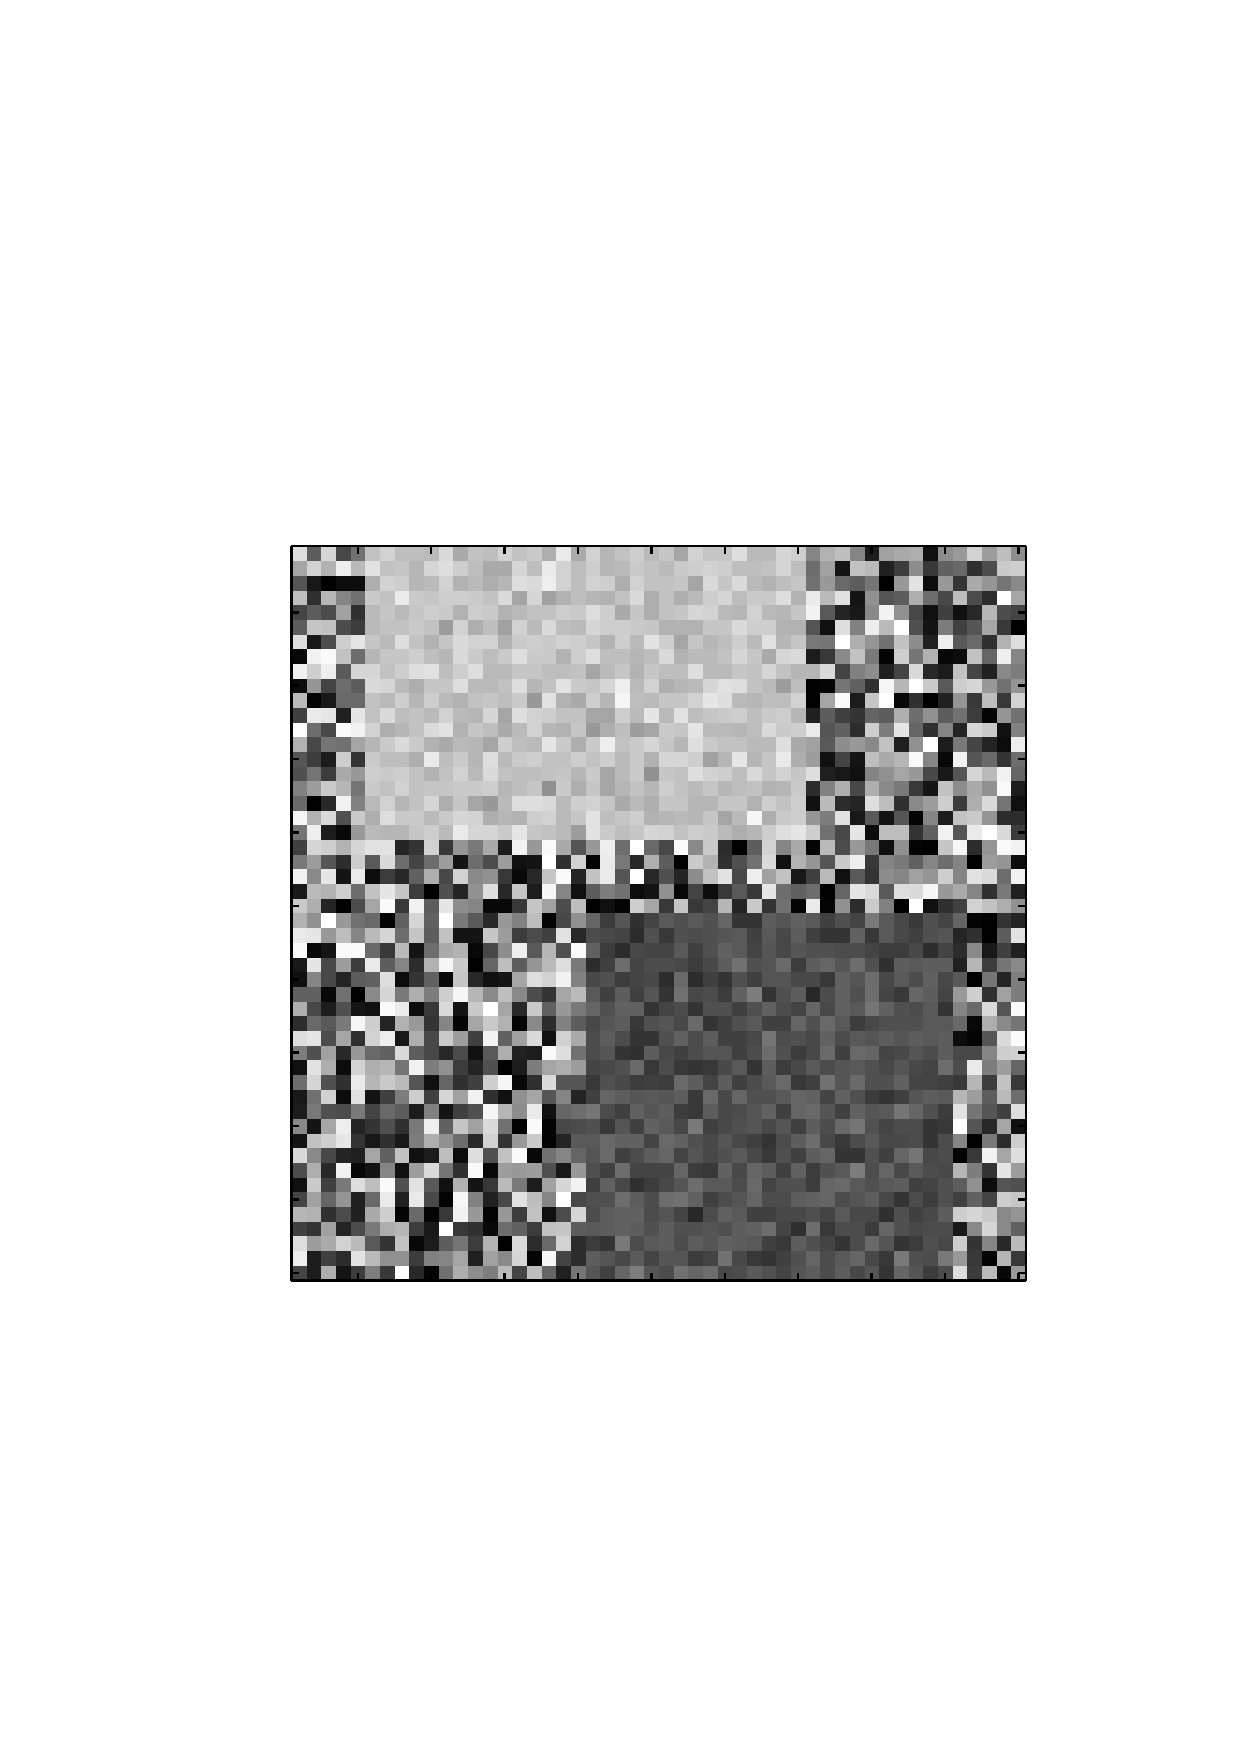
\includegraphics[width=36mm]{ori}&
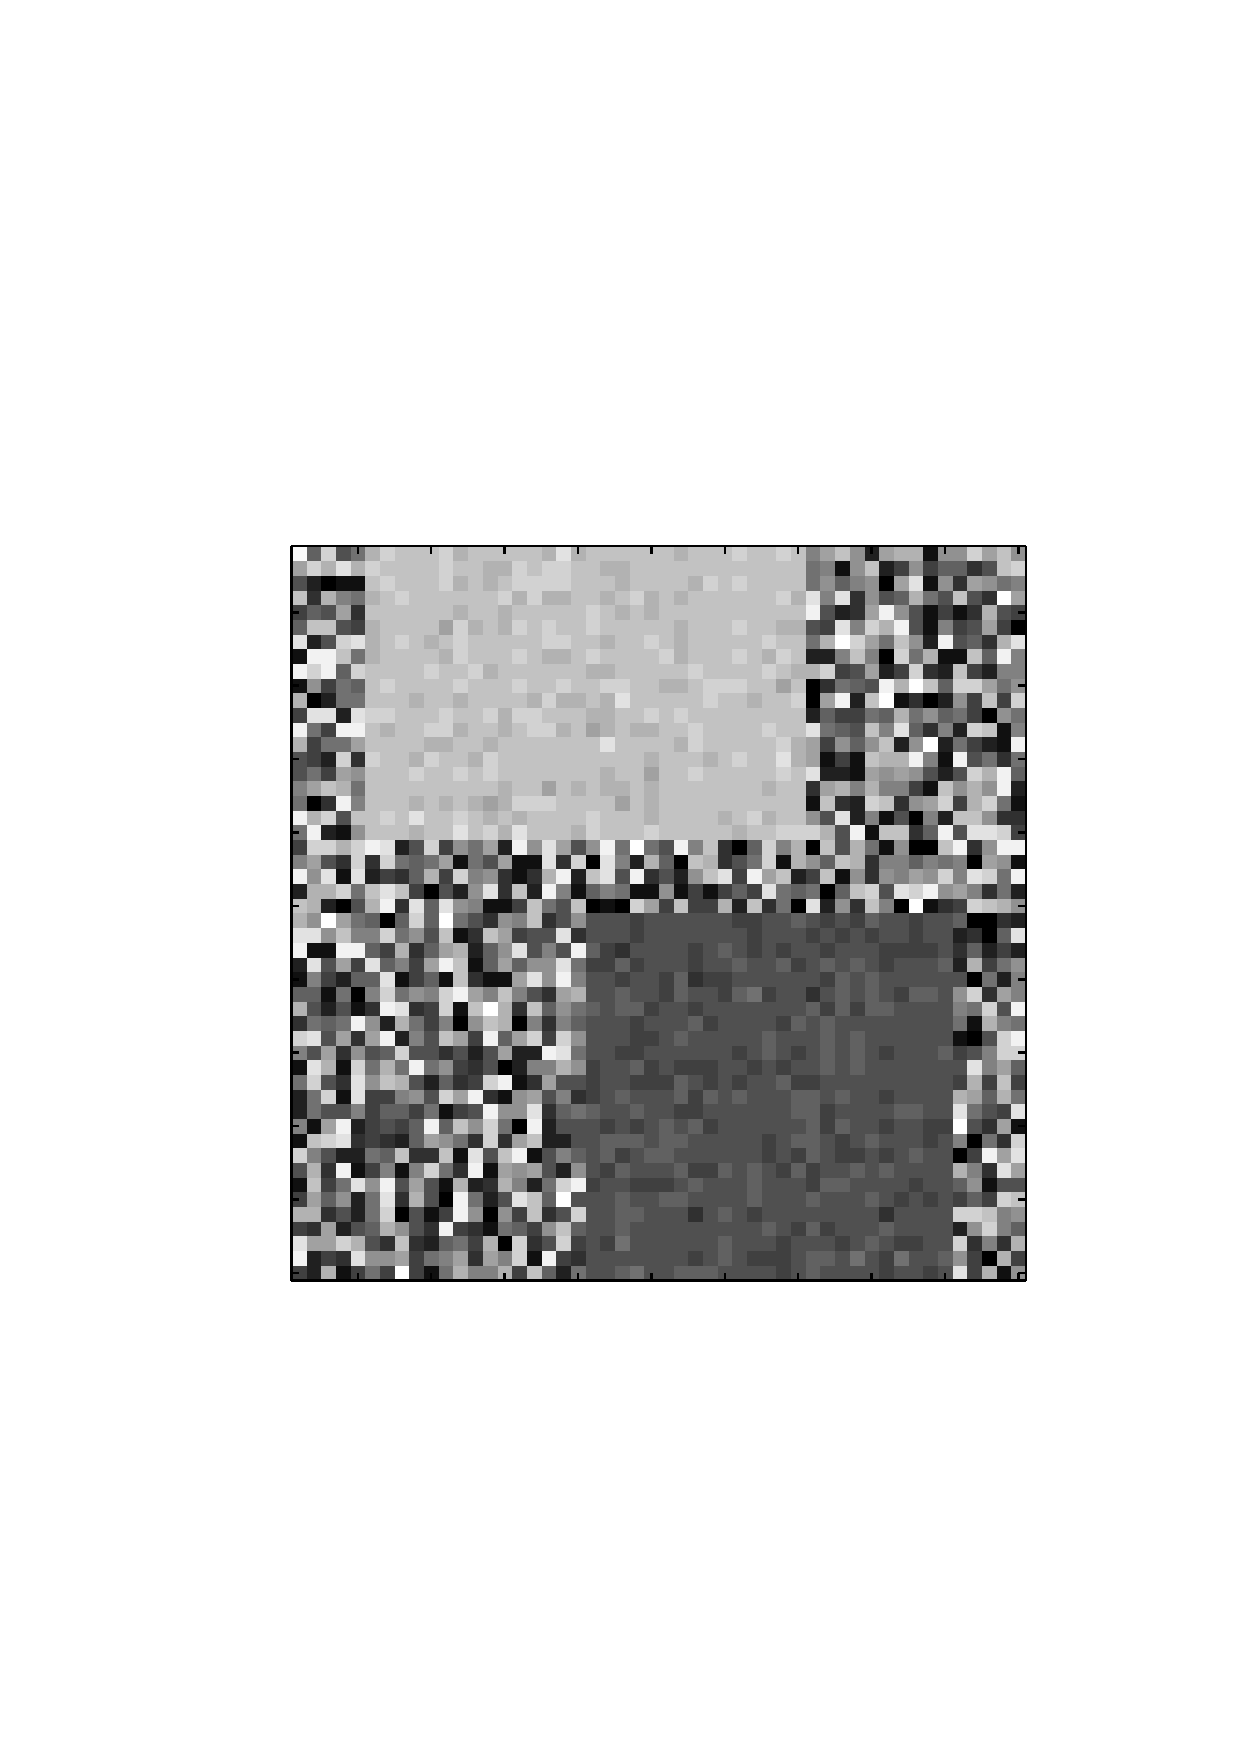
\includegraphics[width=36mm]{lp1}&
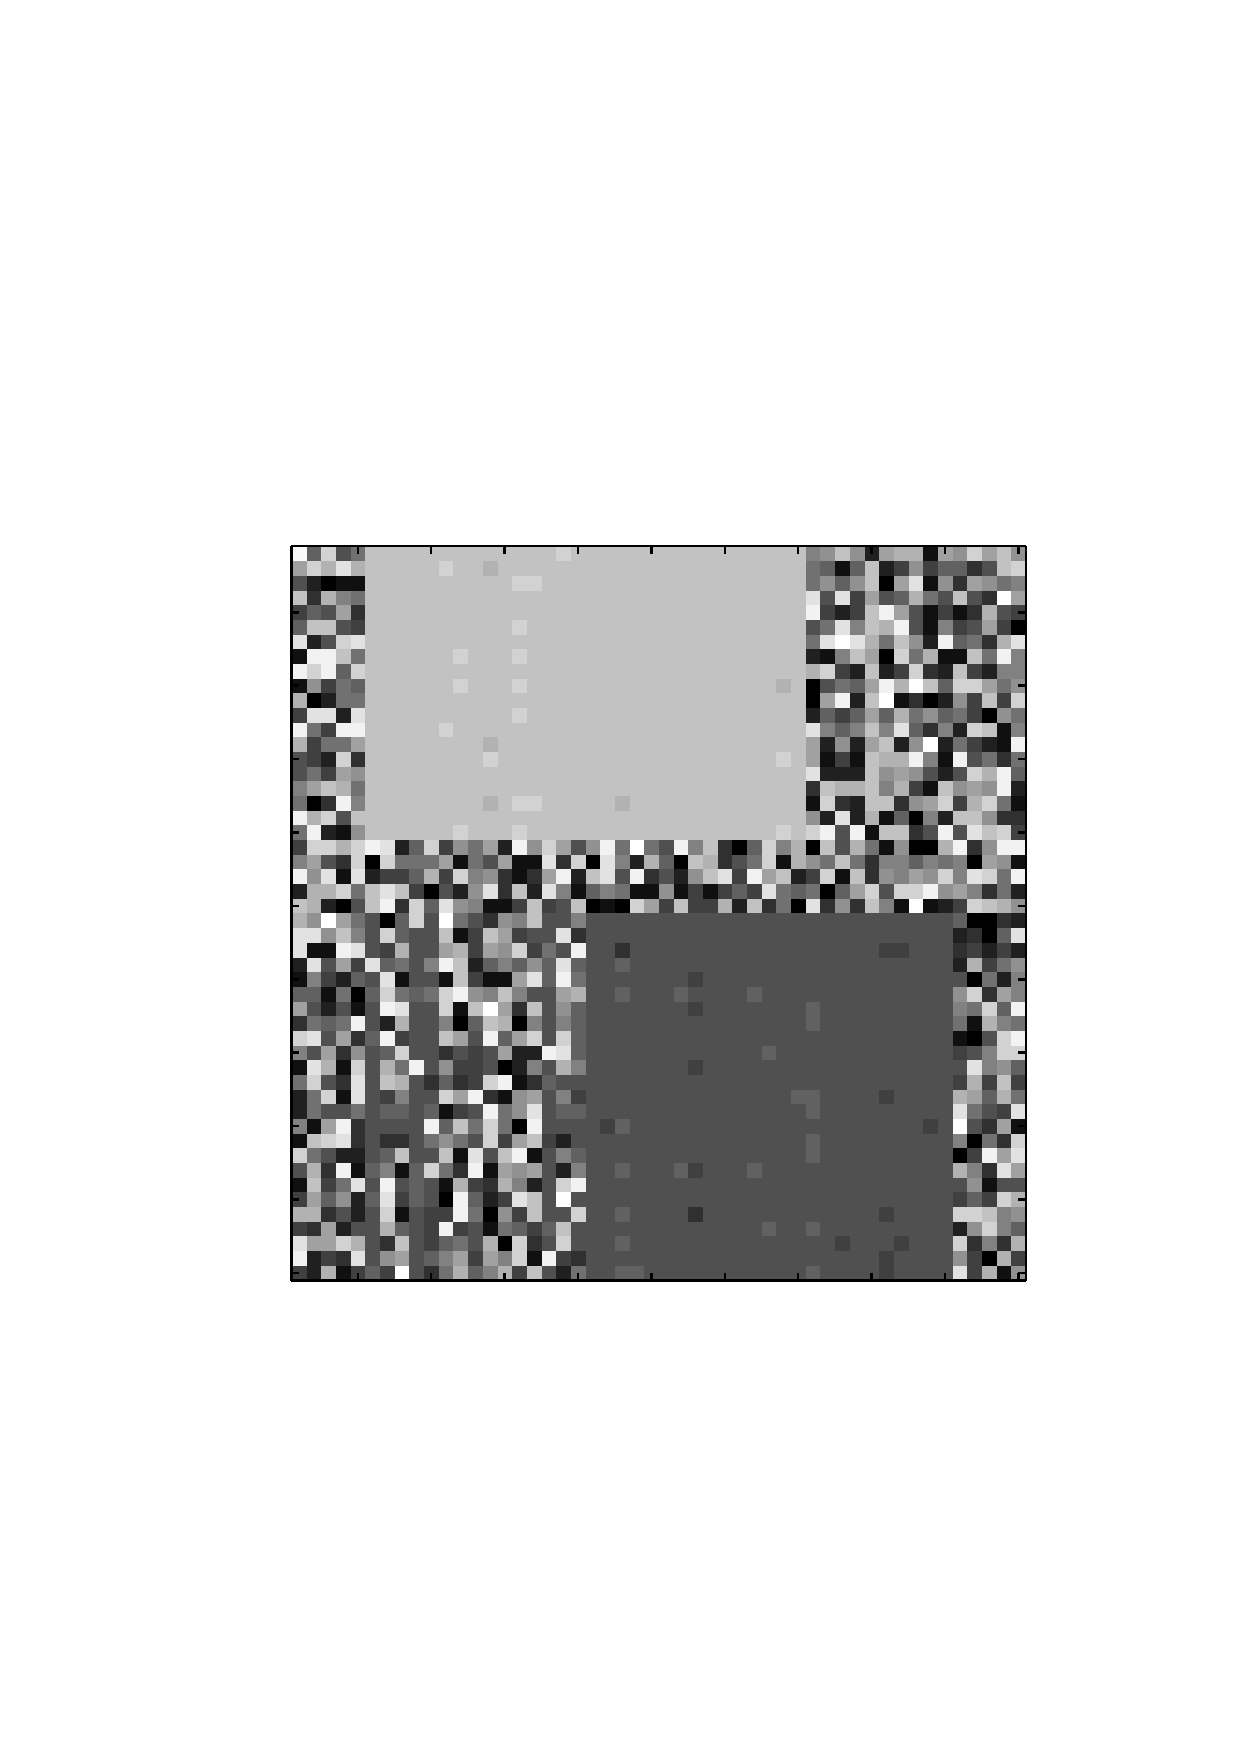
\includegraphics[width=36mm]{lp5}&
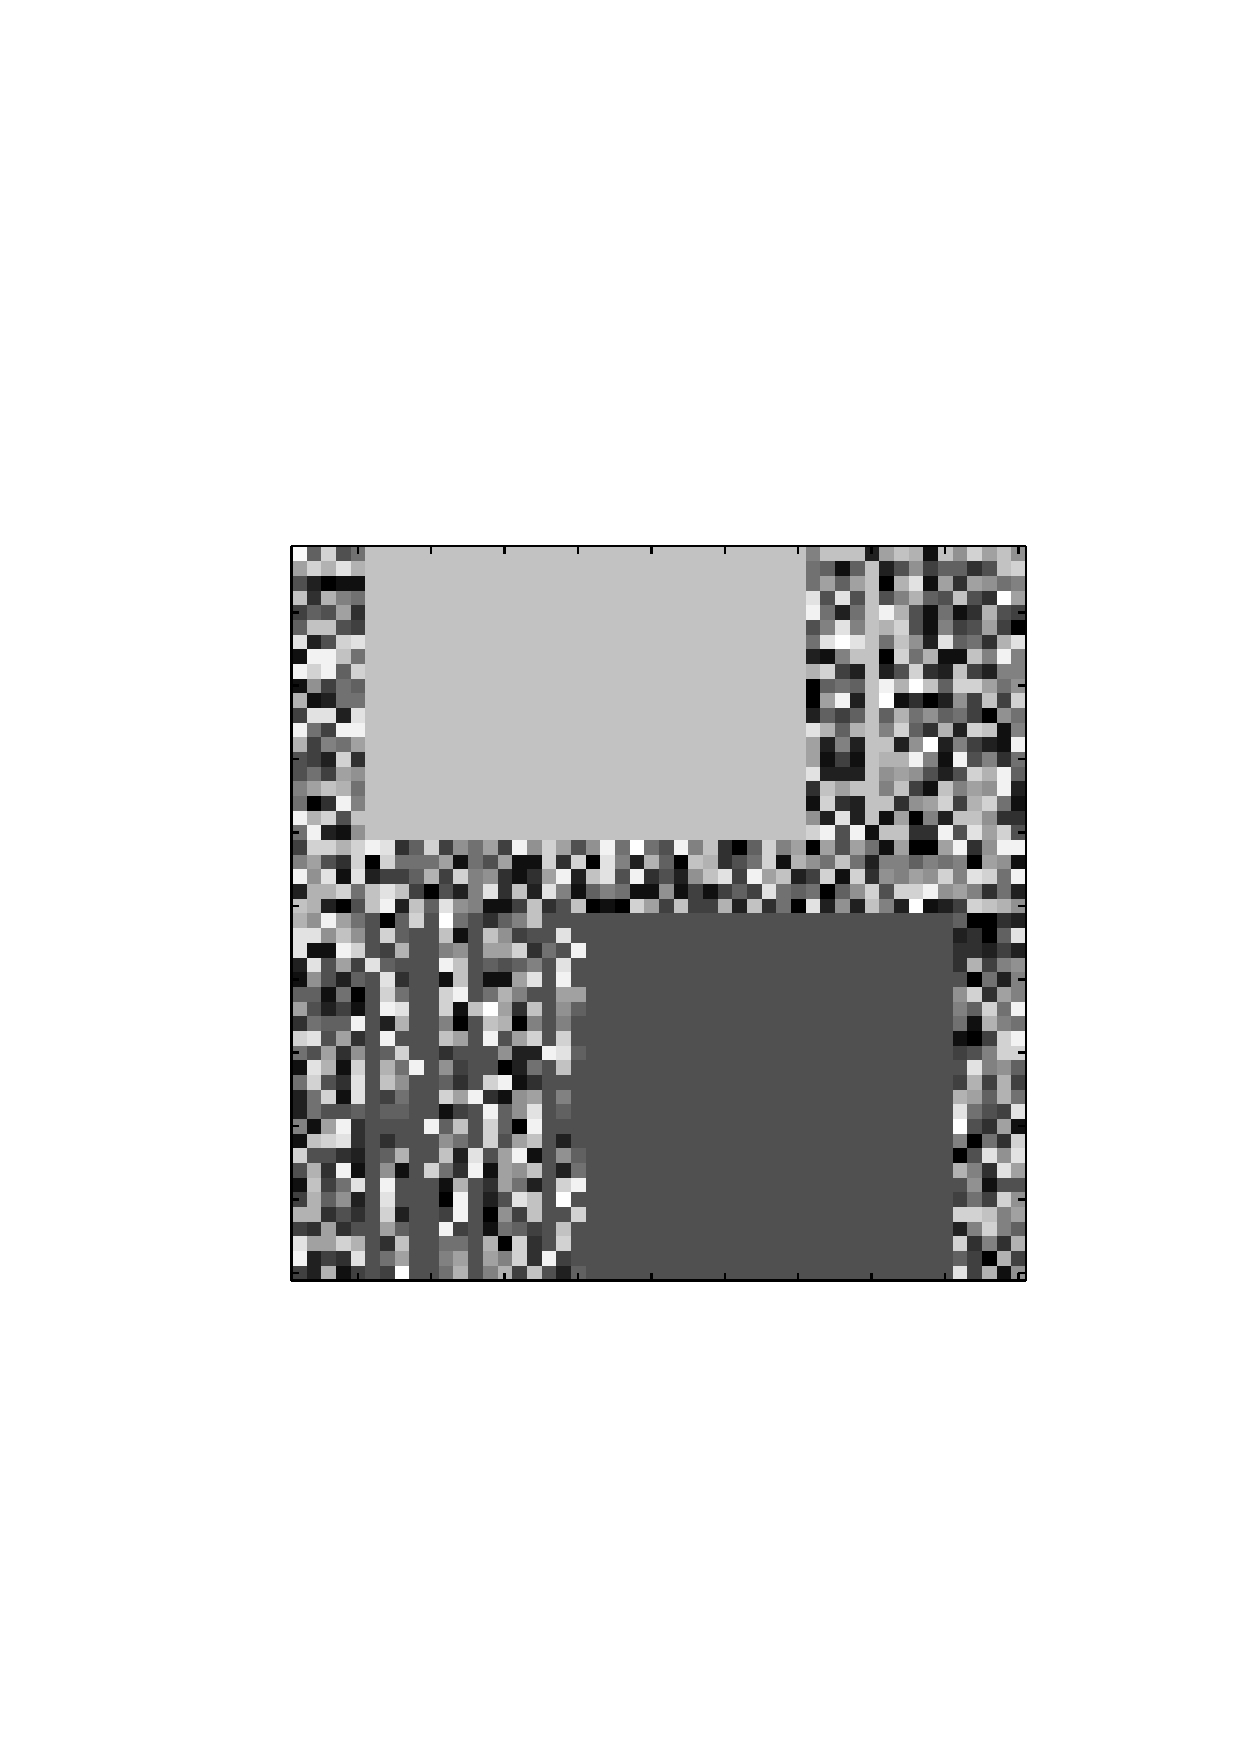
\includegraphics[width=36mm]{lp50}\\
(a) 原始矩阵 & (b) T = 1 & (c) T = 5 & (d) T = 30
\end{tabular}
\caption{\cosync算法动态双边交互过程图。 (a)原始矩阵及包含在其中的两个联合簇。(b)-(c)动态交互在的过程,可以看出联合簇中的值随着时间渐渐同步。(d)算法收敛的同步矩阵,可以看到两个嵌入的聚类簇被完美地发掘出来。}
\label{fig:simulation}
\end{figure*}

可以看出图中两个联合簇的轮廓,需要注意的是,产生这种可见“轮廓”的原因是为了可视化方便而设置的,当矩阵的行、列顺序被打乱后,联合簇将无法被肉眼识别出来,但行、列顺序并不影响\cosync算法的工作。

\vspace{2mm}
图\ref{fig:simulation}(b)-(d)展示了\cosync算法的工作流程。$T$代表双边交互模型的迭代次数,可见在$T=5$次迭代处,联合簇的轮廓就已经逐渐清晰。往后的迭代中,收敛速度逐渐变慢,直到进行到30次,同步因子的改变量小于一定阈值,停止迭代得到收敛的同步矩阵。原始的两个联合簇都被完整地挖掘出来。图\ref{RC}展示了这一过程中同步因子$r$的收敛过程。
\vspace{2mm}
\pic[htb]{同步因子随时间收敛图}{width=80mm}{RC}

从图中可以看到同步因子将收敛于$1$,且其收敛的速度初始很快,随着迭代的进行越来越缓慢,形成一个平稳的曲线。

受限于篇幅的原因,关于更多\cosync在人工数据集上的结果被置于附录中。从这些实验中我们可以得出结论,\cosync算法对于原始矩阵中嵌入的少量大尺寸联合簇的挖掘结果表现良好,受动态同步的思想驱动,嵌入在数据集中的联合簇都被自然地挖掘了出来,且对参数的上下浮动的敏感性较低,具有不错的鲁棒性。但是若在数据集中嵌入的联合簇的分布复杂,且尺寸小数量多的情况下,则受限于相似性度量难以有效发挥作用,不能很好地同步在一起。

\subsection{\cosync与其他算法的性能比较}
\label{subsec:compare}
为了证明我们的算法相对于与其他算法的优势,说明\cosync算法能挖掘出任意排列方式的联合簇,我们设计了两个代表性的$(1000\times1000)$的中大型数据矩阵。其中一个矩阵中的联合簇将以棋盘(checkboard)的方式分布,如图\ref{fig:yiqi}(a)所示;而另一个矩阵中的联合簇位置分布任意,如图\ref{fig:yiqi}(c)所示。图中矩阵里嵌入的颜色深浅不一的子矩阵从均值不一的高斯分布$N(\mu,\sigma)$中采样得到。为了消除行、列的排序对算法性能的影响,图\ref{fig:yiqi}(b)和(d)是棋盘分布矩阵和随机分布矩阵行列顺序打散后的结果。所有的实验都将在乱序上的矩阵上进行。

接着我们将分别在这两个数据矩阵上,用\cosync,ITCC,MSSRCC,Spectral Clustering,Plaid进行测试。国际上很多主流算法由于自身局限性,对数据矩阵有较强的假设:联合簇的分布为棋盘式的,比如本次进行试验的ITCC,MSSRCC和\\Spectral CLustering算法。在这样的假设下,这些算法将分别对行、列空间进行聚类,最后把同一个簇的行列集合放到一起形成子矩阵。此外除\cosync外的四种算法都需要指定双边聚类的行、列各自划分的数目,相当于一个先验参数。下面是两个数据集分别的实验结果:

\vspace{4mm}
\tabcolsep=2pt
\begin{figure*}[!htb]
\centering
\begin{tabular}{cccc}
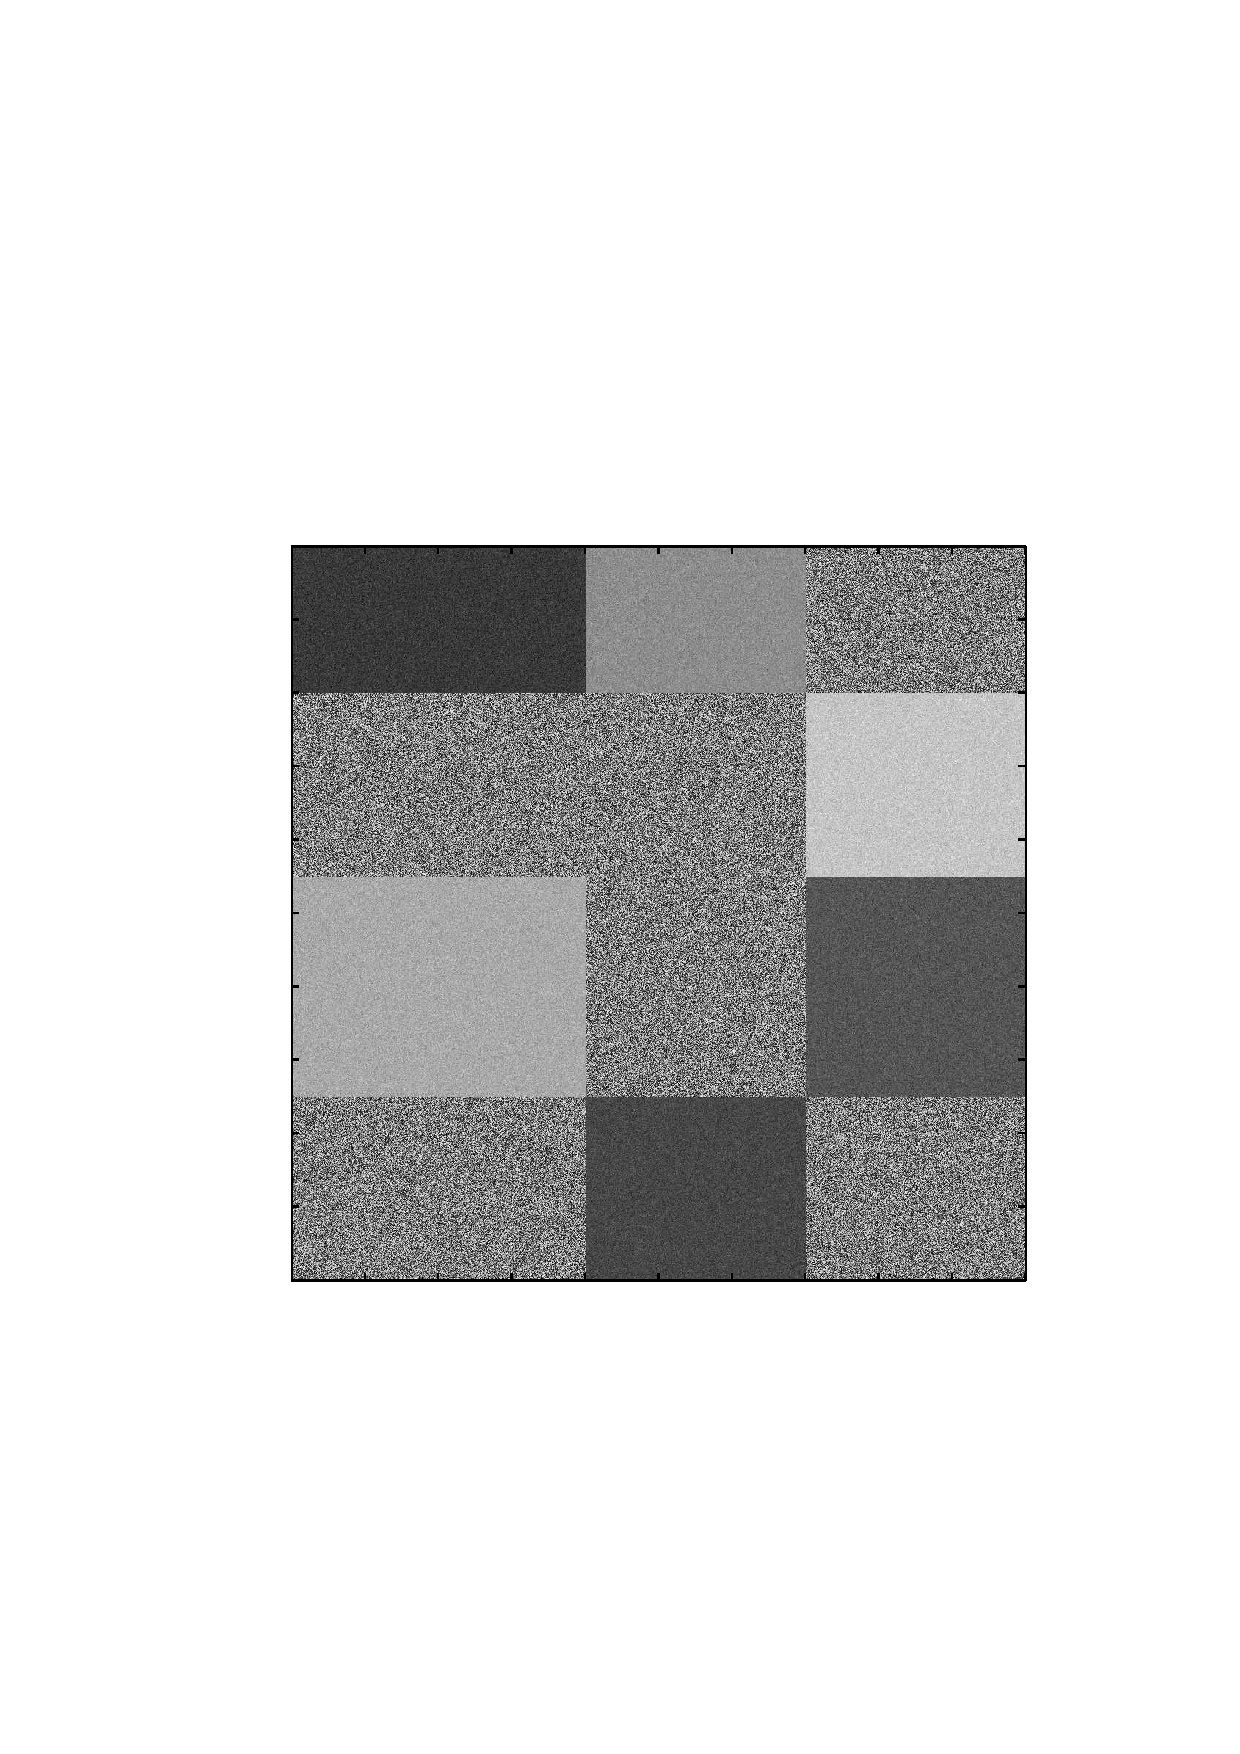
\includegraphics[width=36mm]{O1}&
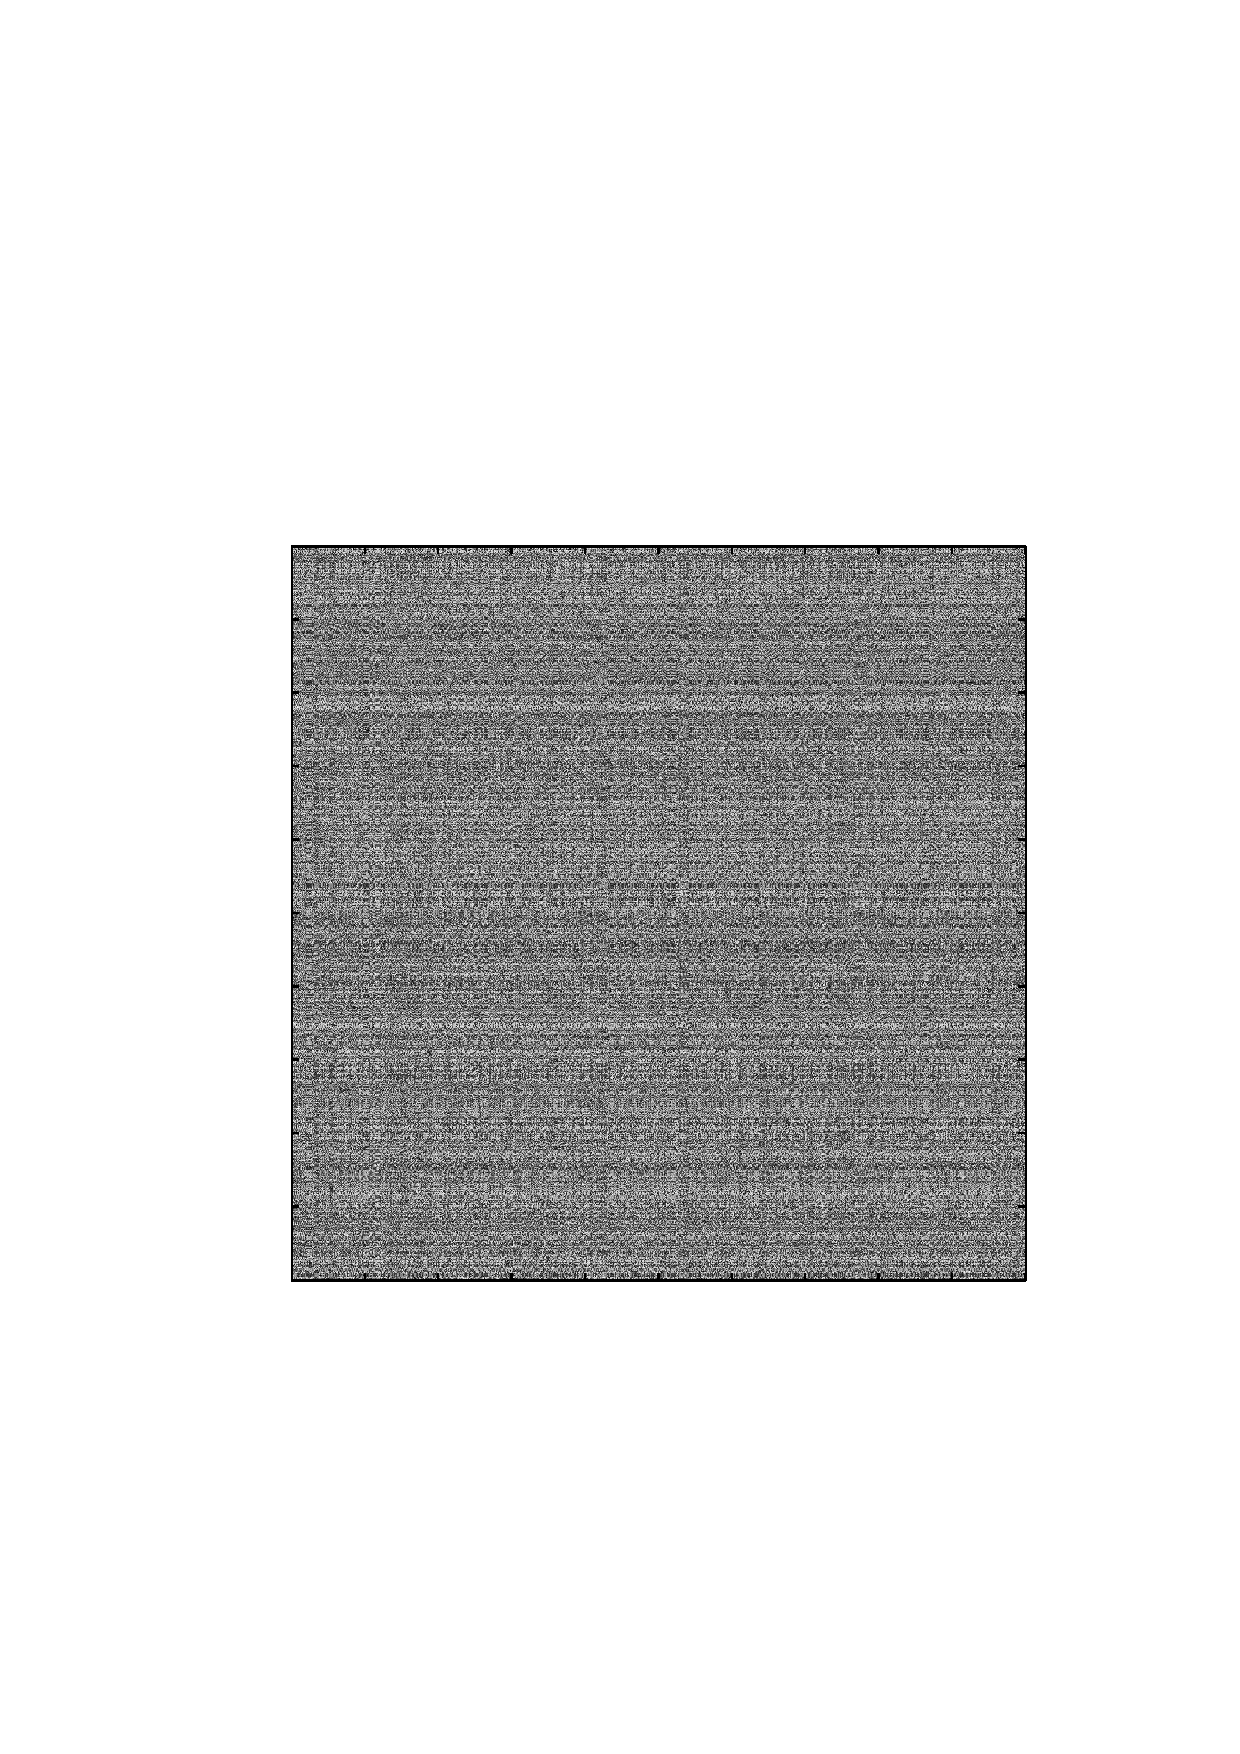
\includegraphics[width=36mm]{S1}&
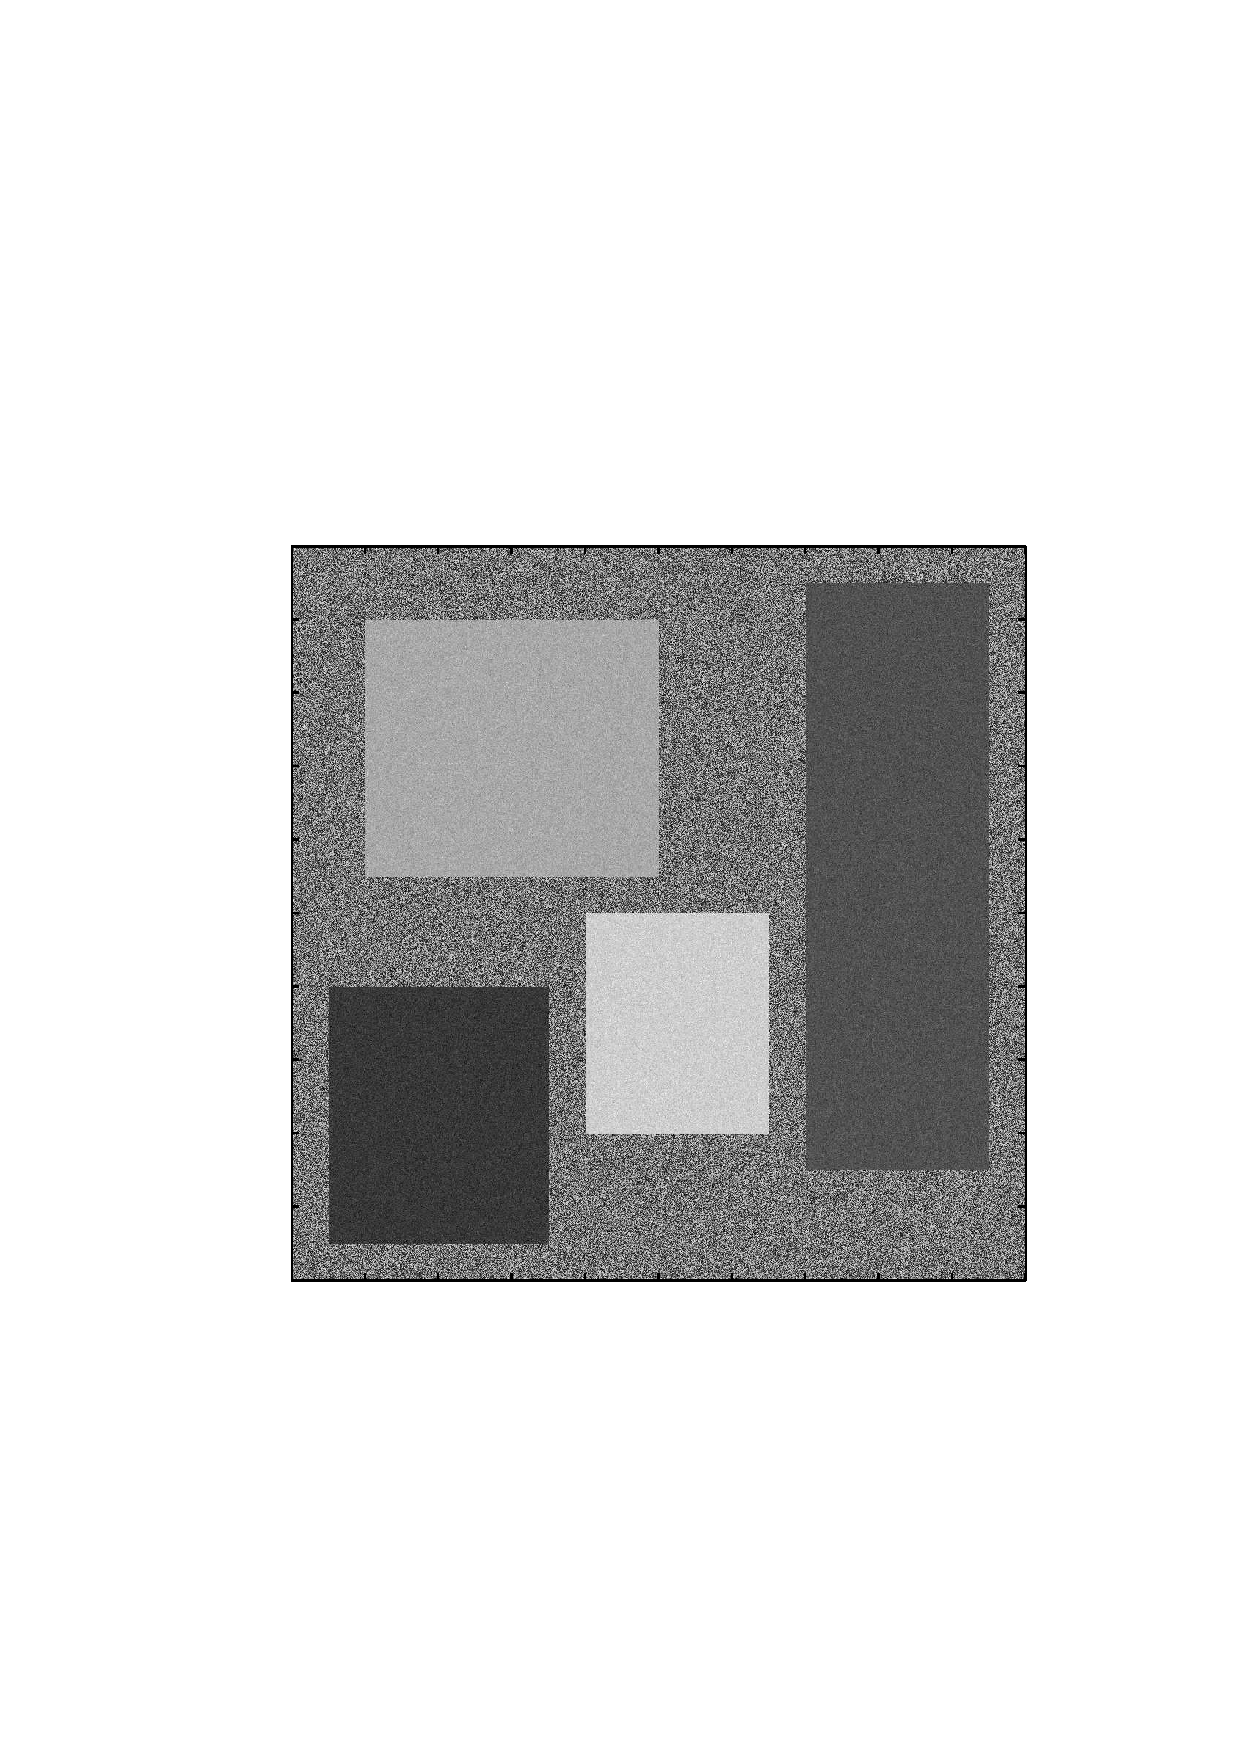
\includegraphics[width=36mm]{O2}&
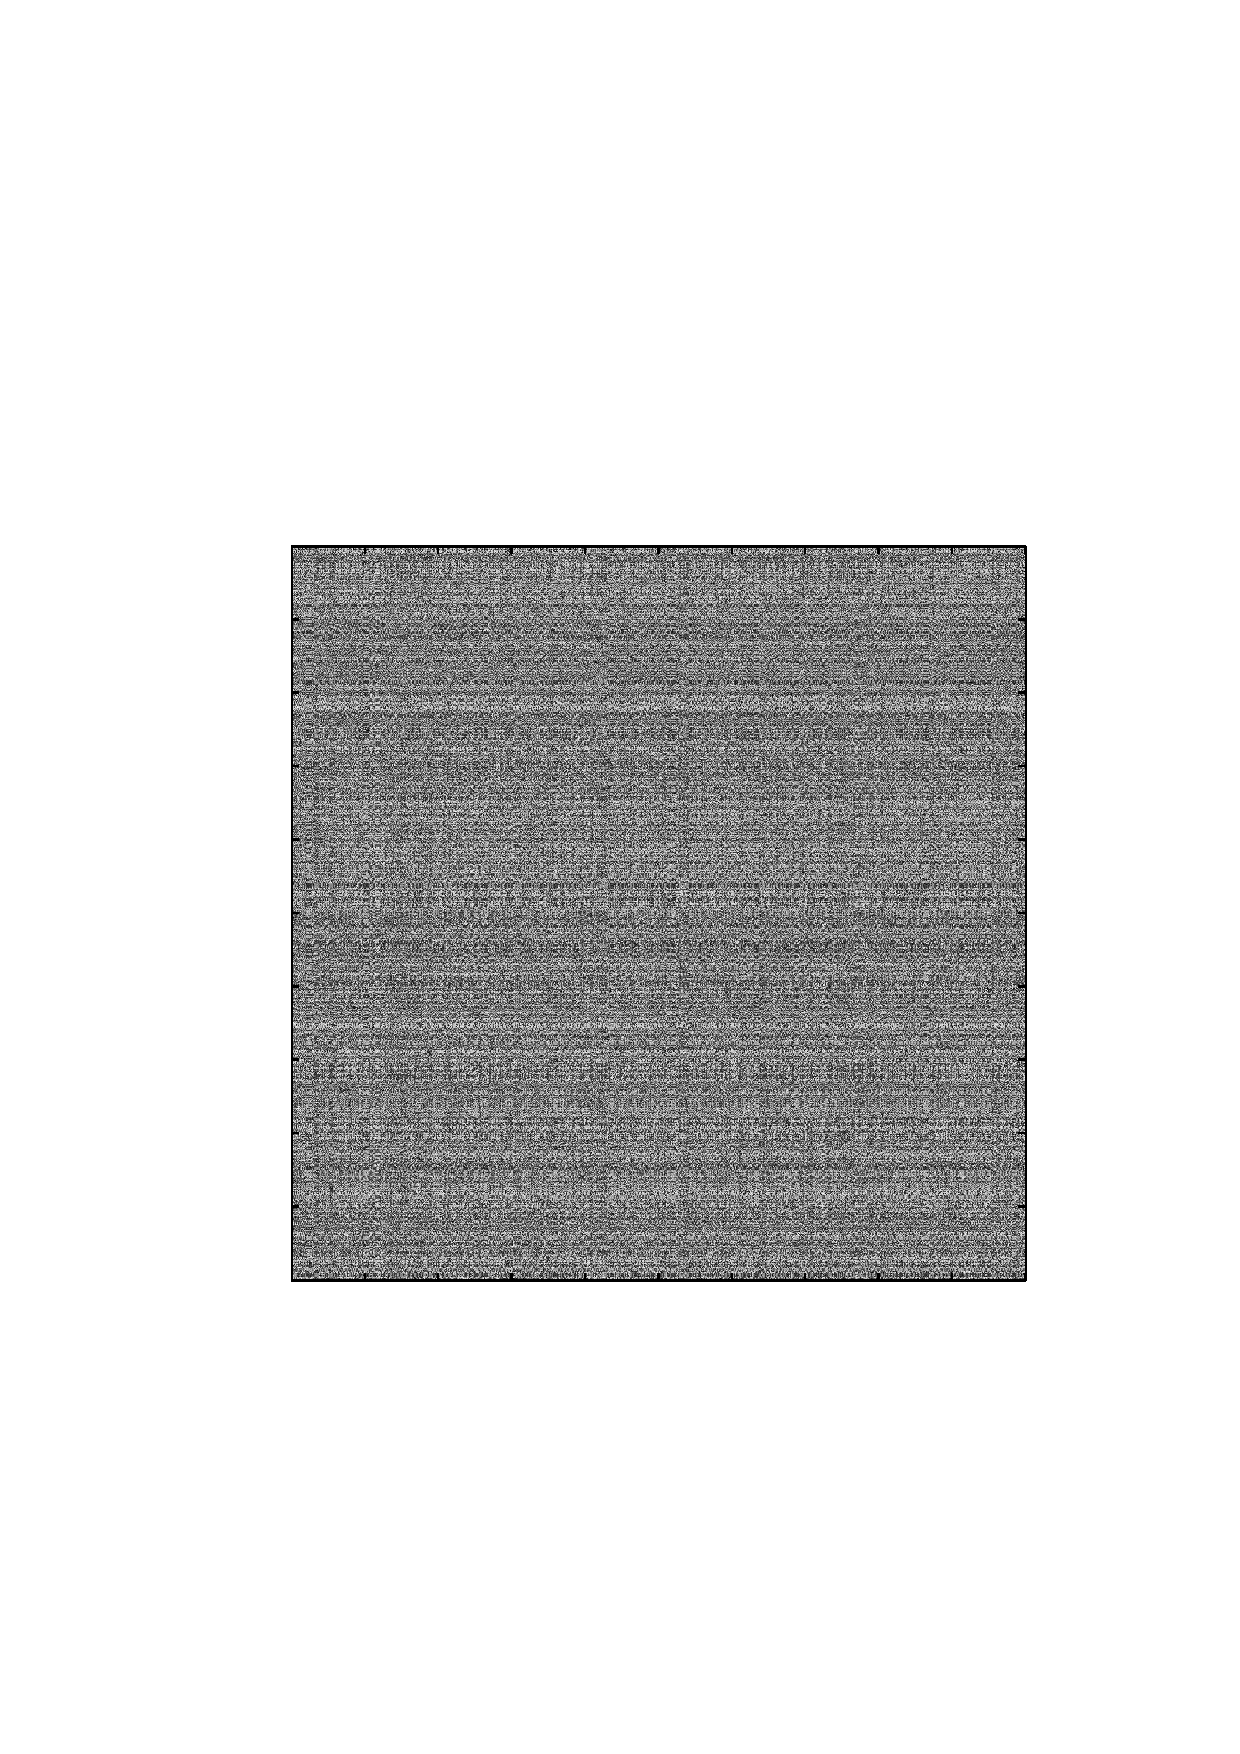
\includegraphics[width=36mm]{S1}\\
(a)棋盘分布矩阵  & (b)棋盘分布行列打散 &(c)随机分布 &(d)随机分布行列打散
\end{tabular}
\caption{棋盘分布矩阵及行列顺序打散矩阵图}
\label{fig:yiqi}
\end{figure*}

\vspace{3mm}
\textbf{棋盘分布下的算法比较}:
在本实验中,首先针对ITCC,MSSRCC和Spectral CLustering算法的特性,对棋盘式分布的矩阵进行测试。实验矩阵尺寸为$(1000\times1000)$,嵌入了6个从均值不同的高斯分布$N(\mu,\sigma)$中抽样的联合簇,其可视化图行列打散的的矩阵如图\ref{fig:yiqi}(a)-(b)所示。由于数据集的分布为棋盘分布,故行、列的划分数目很好确定,分别为$4$与$3$。

在5种算法完成测试后,各自得到输出的代表联合簇的行、列集合。我们对它们进行排序整理,重新规划为易于观察的矩阵,其可视化结果如图\ref{fig:yiqi_r}(b)-(f)所示。

图中红色方框为结果中识别出的聚类簇。可见只有\cosync和Plaid算法能够识别分散在矩阵中的聚类簇,其他三种对聚类簇的识别都是基于全局划分的。在图\ref{fig:yiqi_r}(b)中,可见\cosync算法分毫不差地挖掘出嵌入原始矩阵的6个联合簇,做到了识别度$100\%$;而在图\ref{fig:yiqi_r}(f)中,Plaid模型识别出了6个聚类簇中的4个,识别度为$66.6\%$。ITCC、MSSRCC与Spectral Clustering算法用划分的方式将原矩阵划分为$4\times3=12$块,图\ref{fig:yiqi_r}(c),(e)中ITCC和Spectral Clustering的12块子矩阵中成功地包括了嵌入的6块联合簇,而图\ref{fig:yiqi_r}(d)中的MSSRCC算法的划分没有成功地圈出联合簇。

总体来看,在这个实验集上,\cosync表现出了良好的特性,甚至胜出了专为棋盘式数据设计的ITCC,MSSRCC和Spectral Clustering算法。

\vspace{3mm}
\textbf{随机分布下的算法比较}:
在现实数据中,联合簇的嵌入不可能按照棋盘式方式规律分布,其分布是无规律而杂乱的。我们在本次实验中模拟了这种情况,将4个大小、尺寸不一致的联合簇随机嵌入$(1000\times1000)$的矩阵中,注意联合簇间不能互相遮挡重叠。其可视化图行列打散的的矩阵如图\ref{fig:yiqi}(c)-(d)所示。

同样地,5种算法在该数据集上运行完毕后,我们对各自输出的结果矩阵行列顺序整理重排,其可视化结果如图\ref{fig:yiqi_r}(h)-(l)所示。从结果中可以看出,\cosync算法依然准确地识别出了4个嵌入的联合簇,而Plaid算法仅识别出了1个联合簇。值得注意的是,在图\ref{fig:yiqi_r}(i)-(k)中的ITCC,MSSRCC和Spectral Clustering三种基于划分的方法此时已经失去效果。ITCC和Spectral Clustering仅划分出了一个联合簇。但由于受于方法本身的限制,它的划分不能将其余联合簇划分出来。MSSRCC则没有划分到正确的聚类簇。

在这次的比较中,\cosync发挥了其优势:能处理以任何分布方式的聚类簇,且发掘效果显著,胜出了其余几种代表性方法。

\subsection{人工数据集测试小结}
我们在本节的人工数据集测试中,首先用比较简单的$(100\times100)$数据集证明了\cosync算法的可行性,并作出数据集在同步过程中的变化图。接下来,在联合簇以棋盘方式和任意方式分布中大规模的$(1000\times1000)$数据集上,我们将\cosync算法和国际上比较有代表性的双边聚类算法ITCC,MSSRCC,Spectral Clustering和\\Plaid算法进行比较。两个的比较的结果中,\cosync都成功地识别出了矩阵中嵌入的所有联合簇,而其他算法都没有做到这一程度,这充分显现了\cosync算法在这一类数据集上的优势。总体来看,本次实验展示了\cosync算法的高效性和能抓住数据集本质结构的特性。

\tabcolsep=1pt
\begin{figure*}[!p]
\centering
\begin{tabular}{ccc}
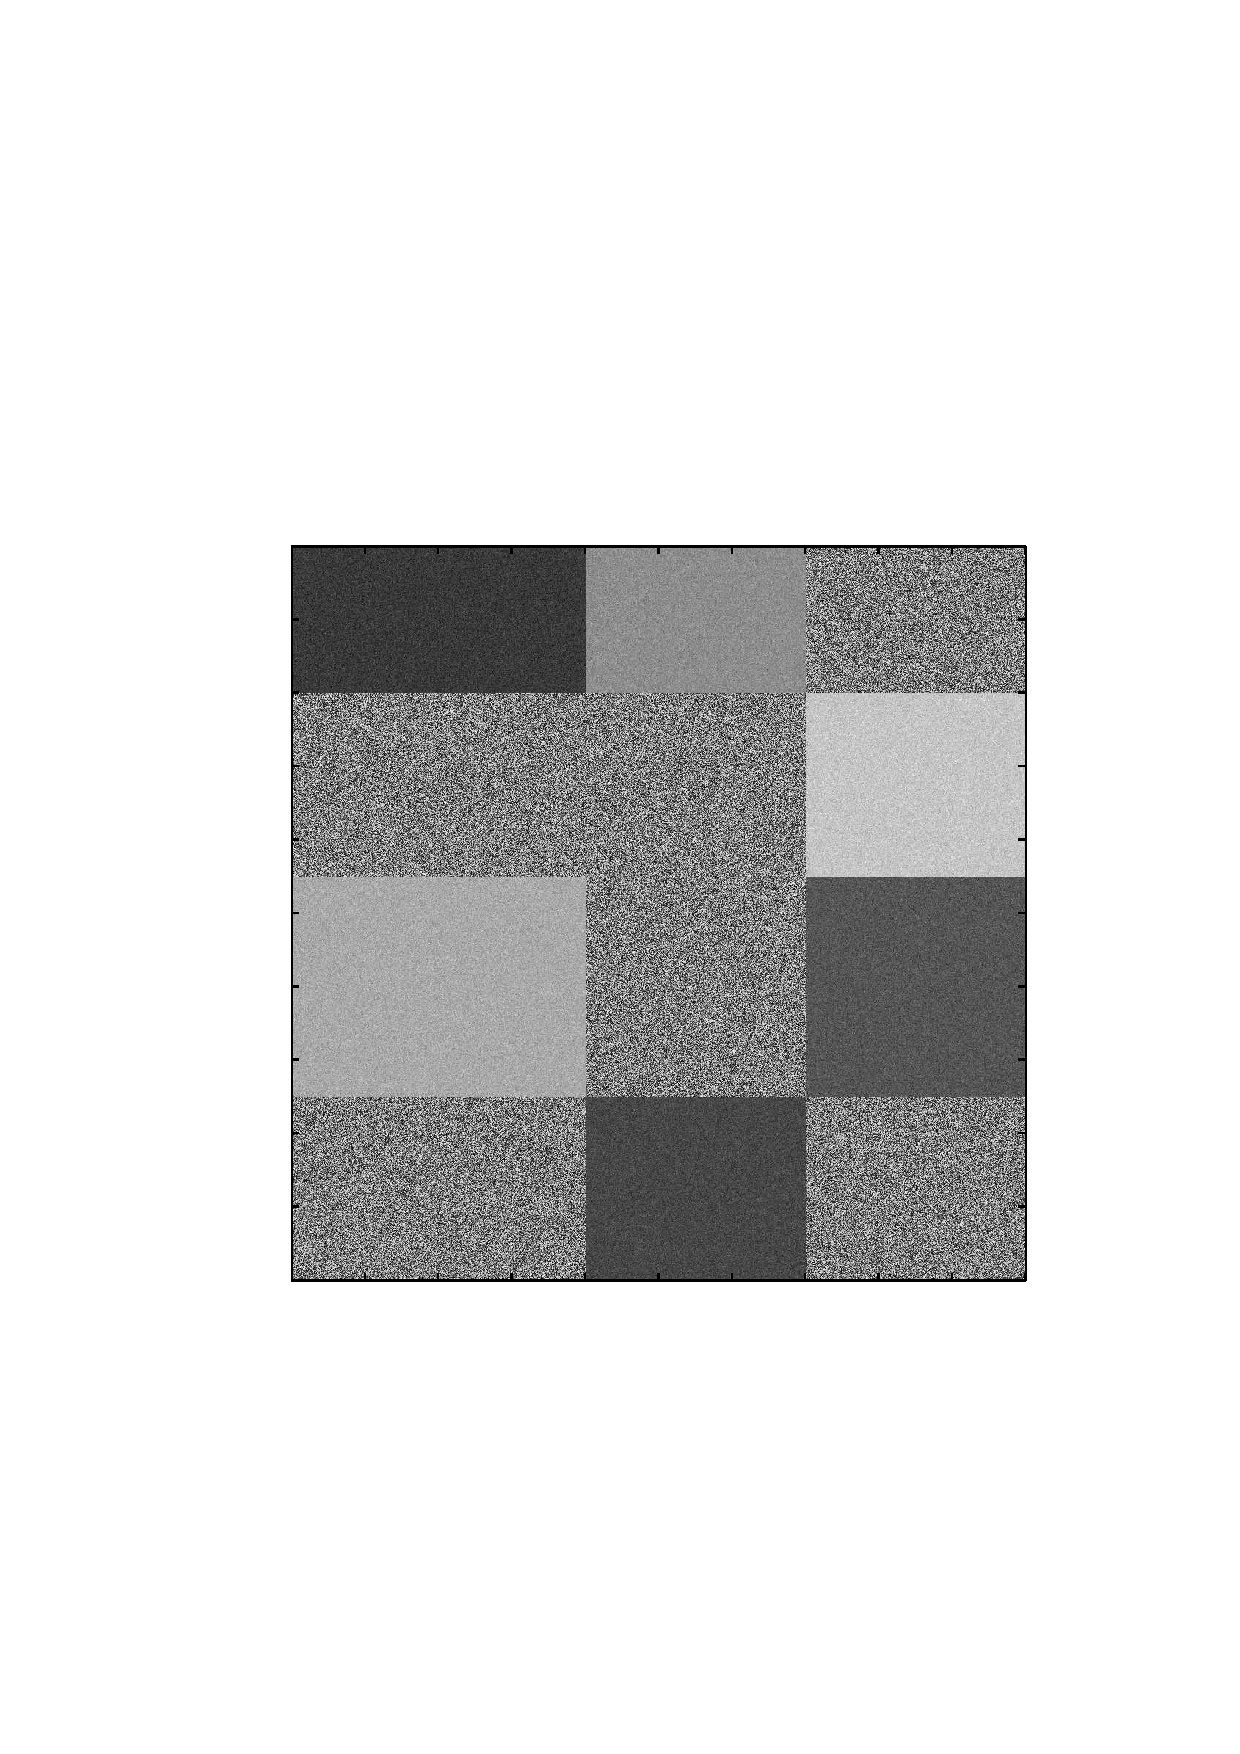
\includegraphics[width=45mm]{O1}&
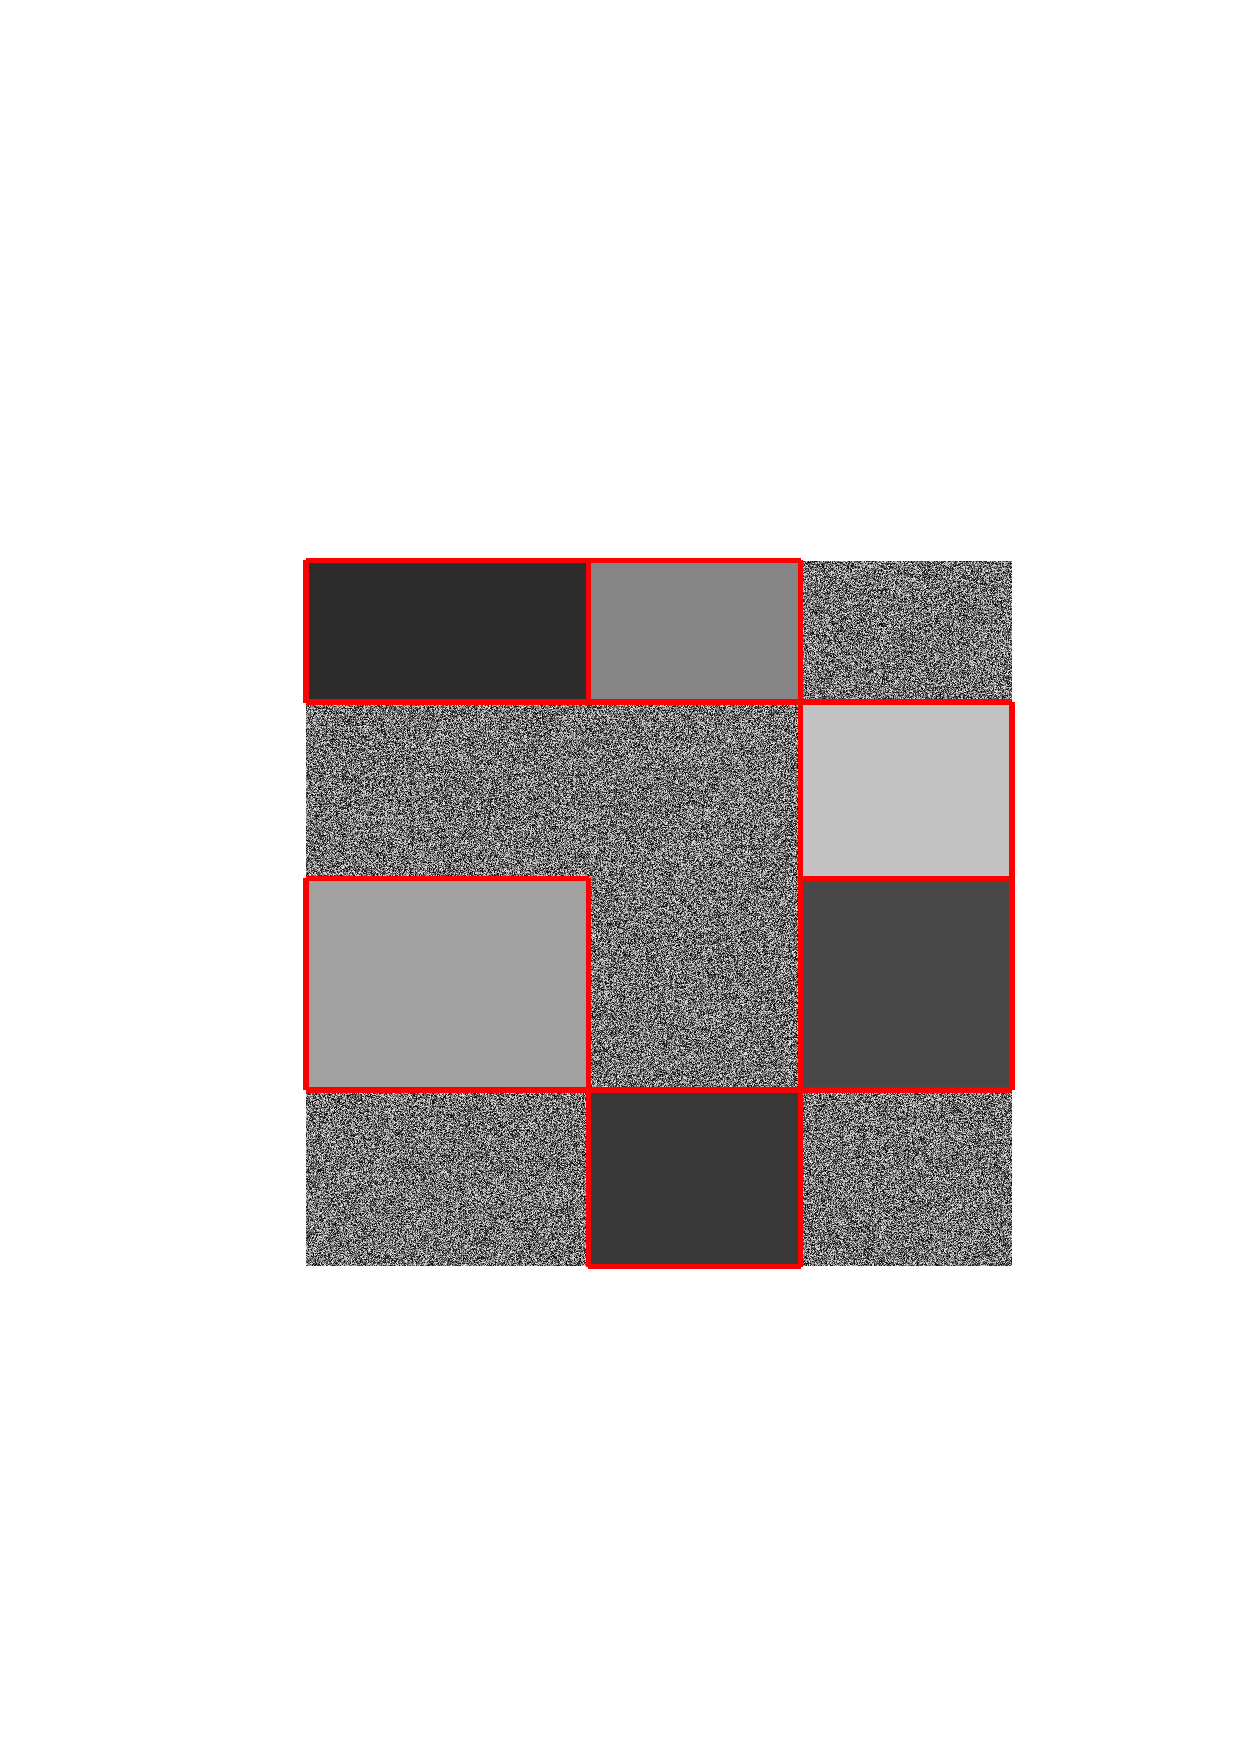
\includegraphics[width=45mm]{syn1R}&
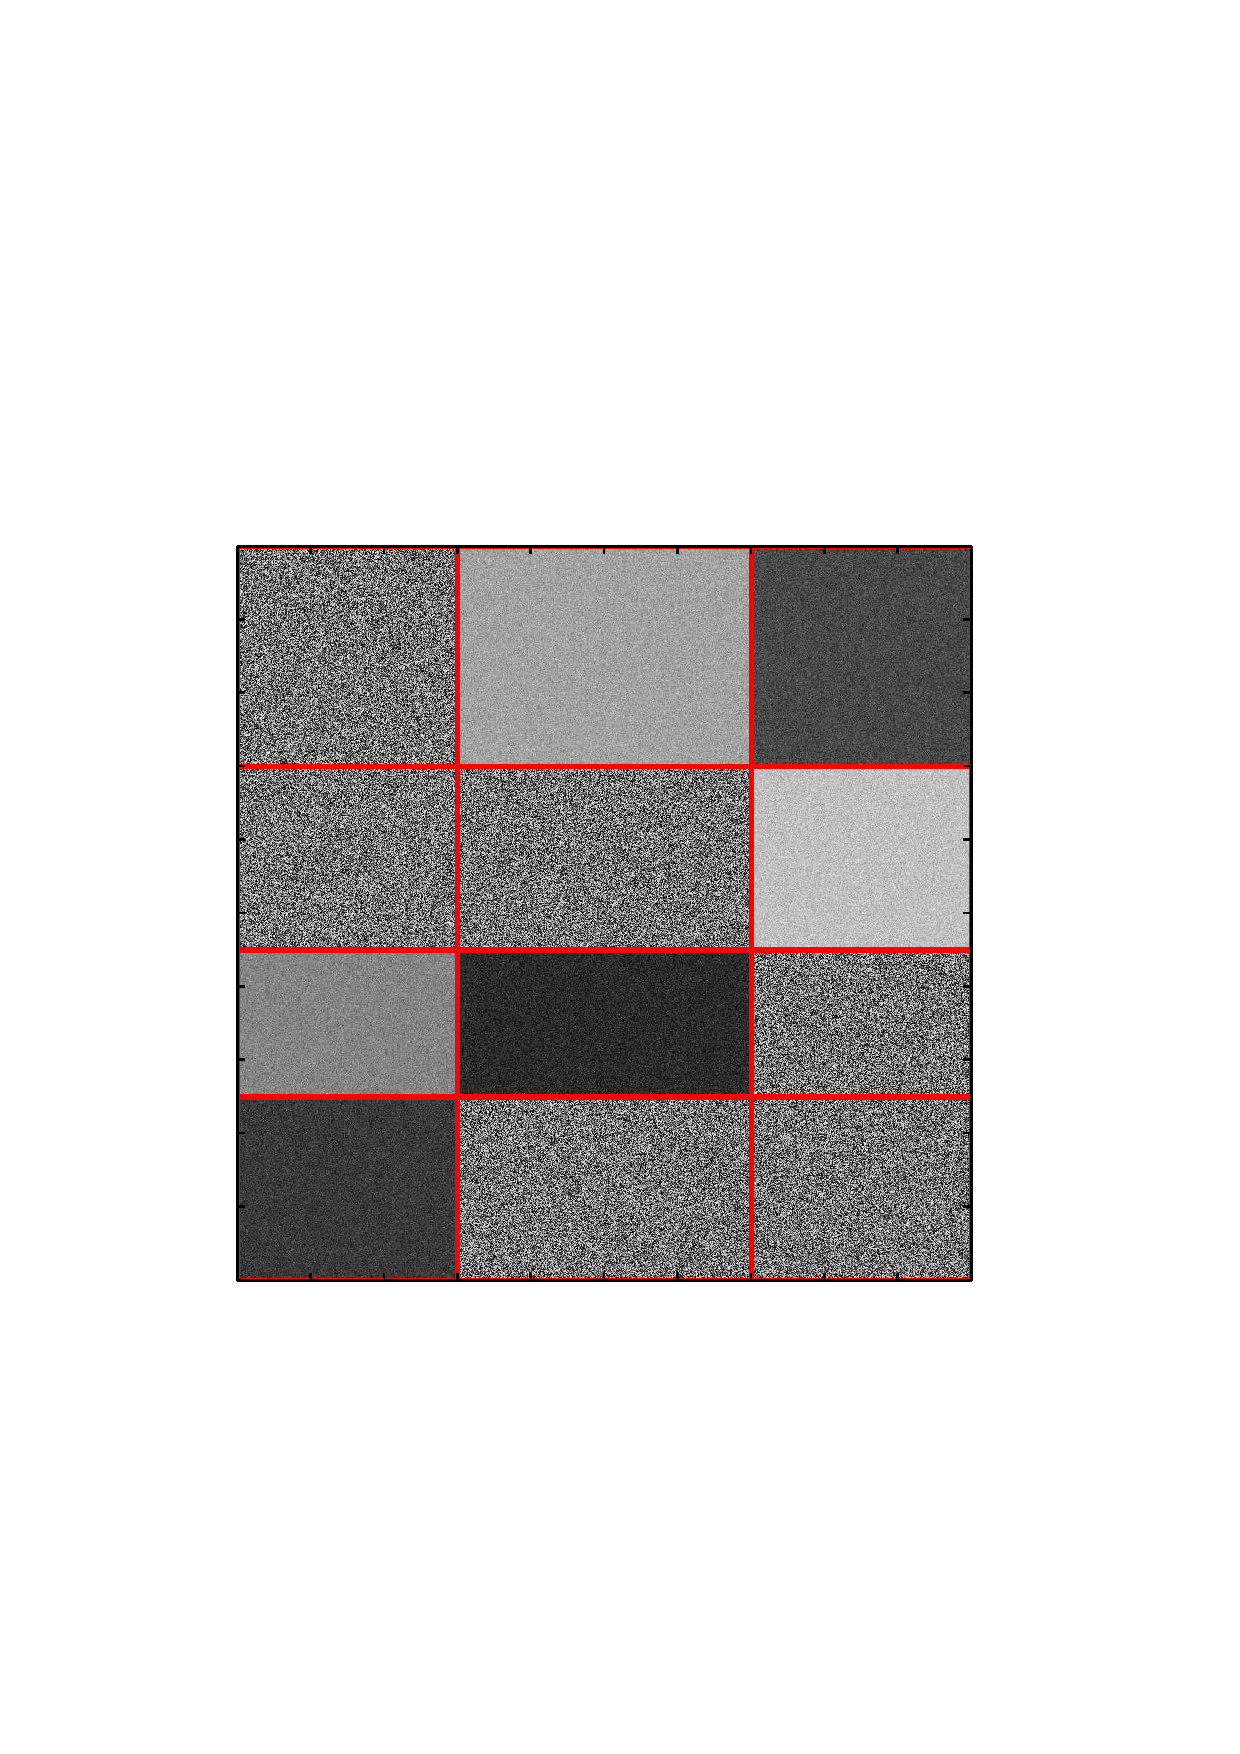
\includegraphics[width=45mm]{inf1}\\
(a) 棋盘分布矩阵  & (b) CoSync &  (c) ITCC\\
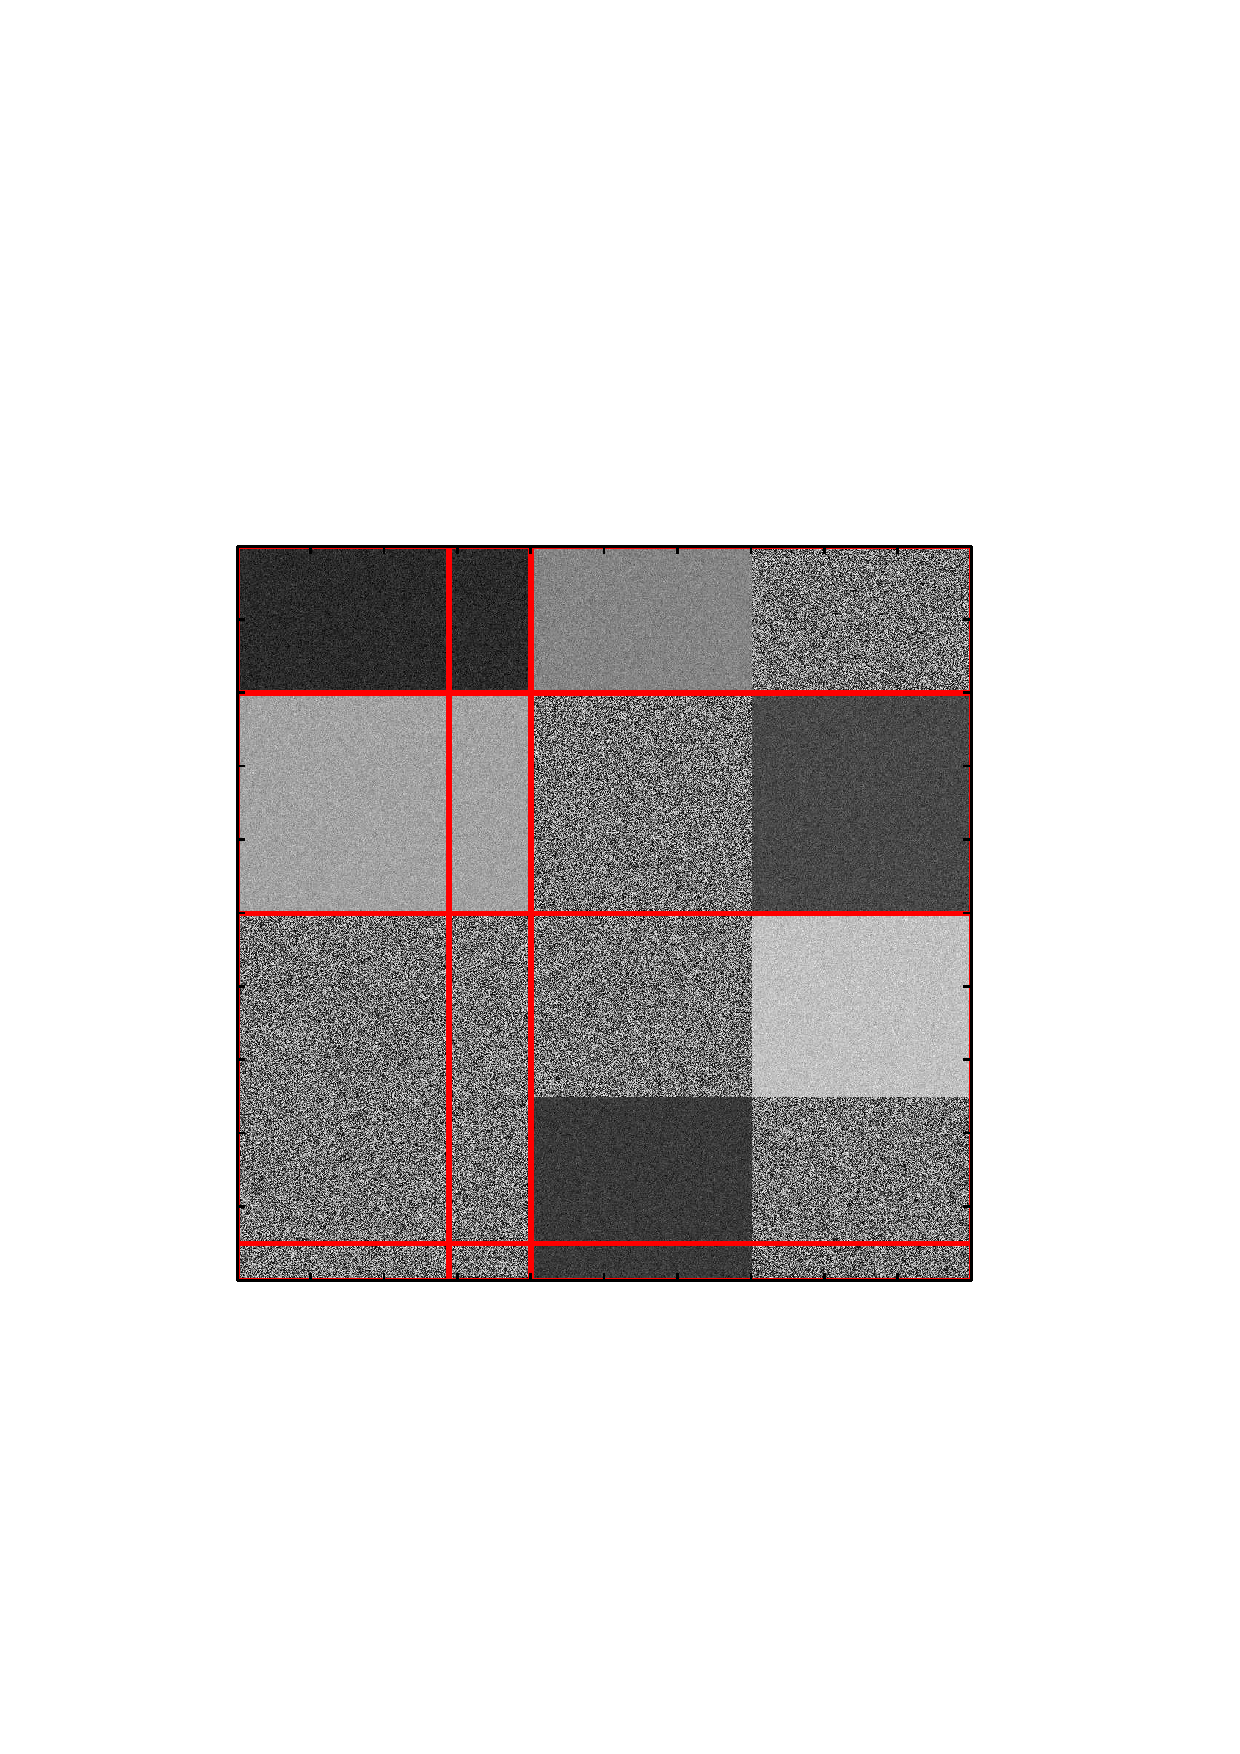
\includegraphics[width=45mm]{residue1}&
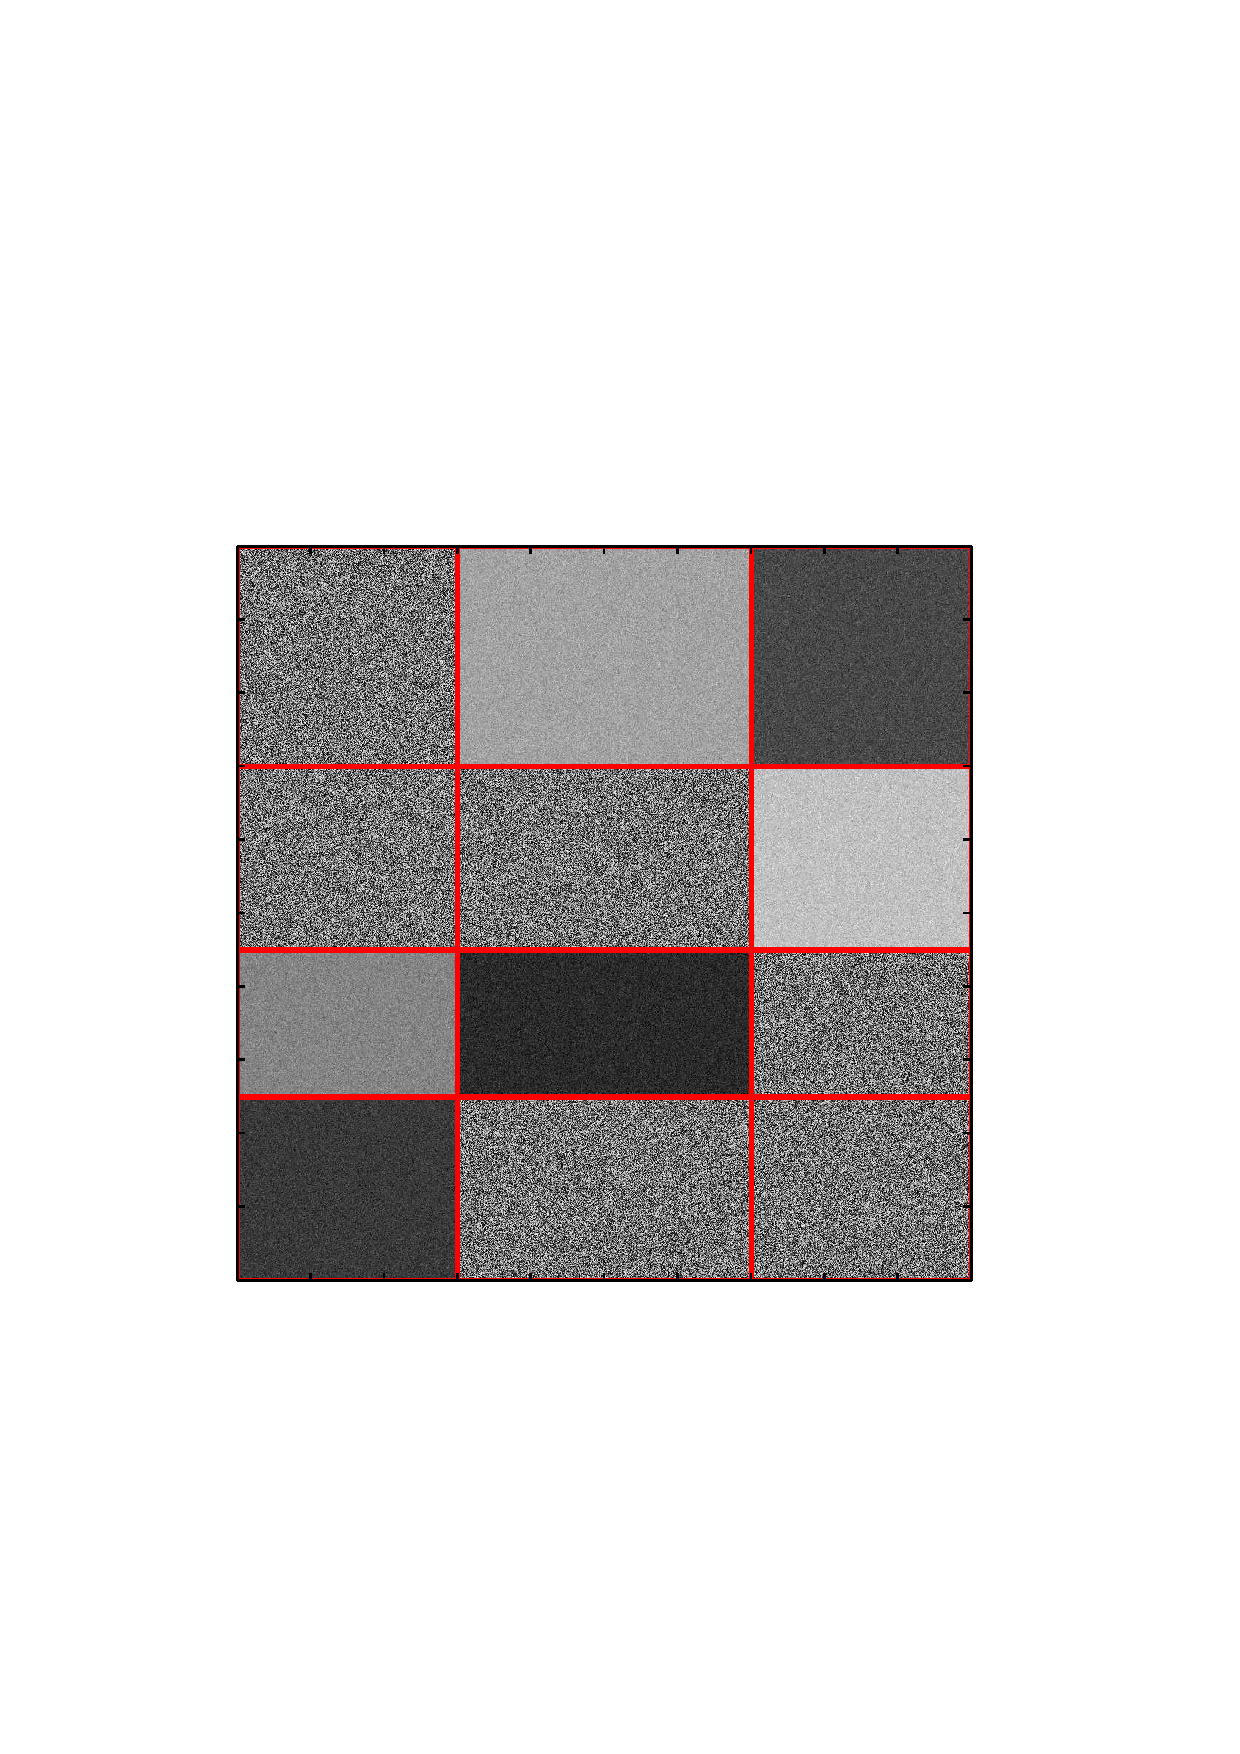
\includegraphics[width=45mm]{spectral1}&
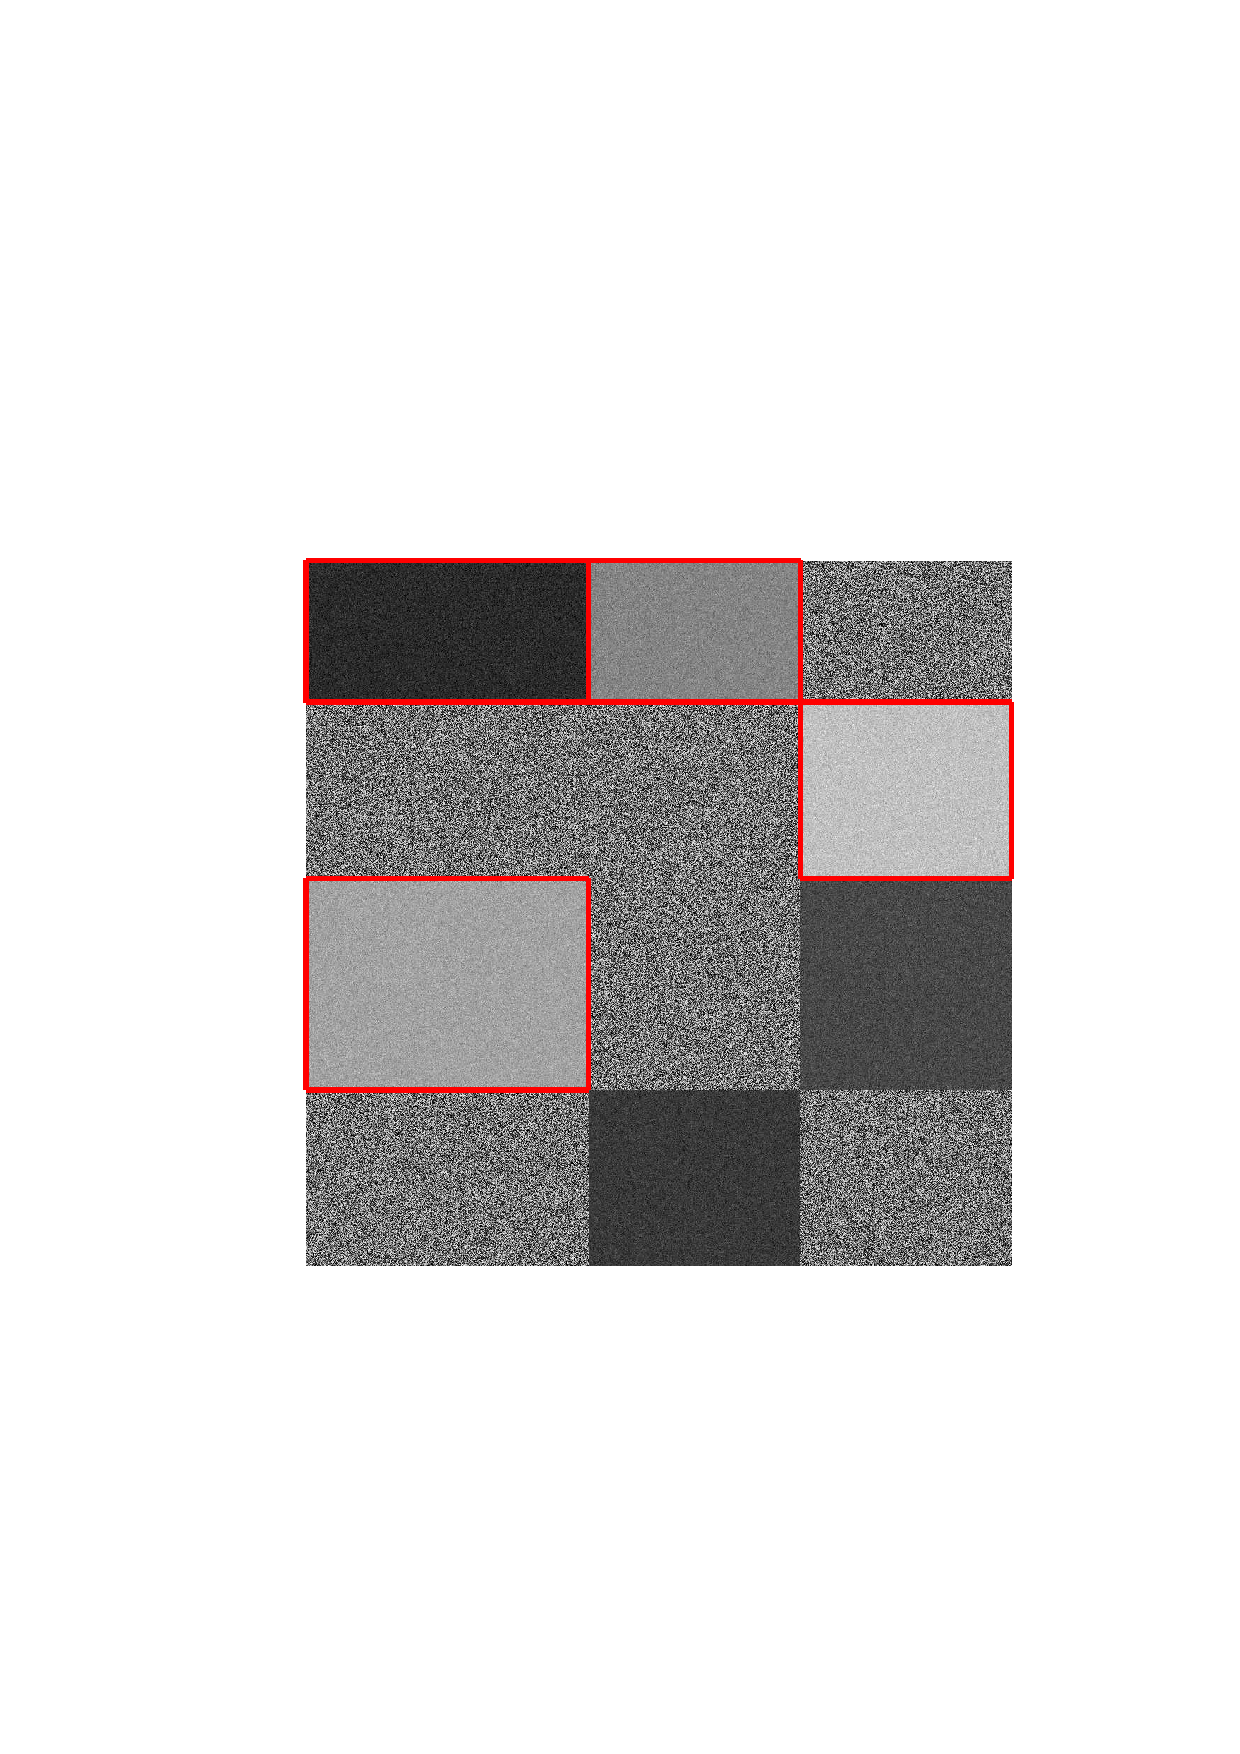
\includegraphics[width=45mm]{plaid1}\\
(d) MSSRCC &  (e)  Spectral &  (f) Plaid\\
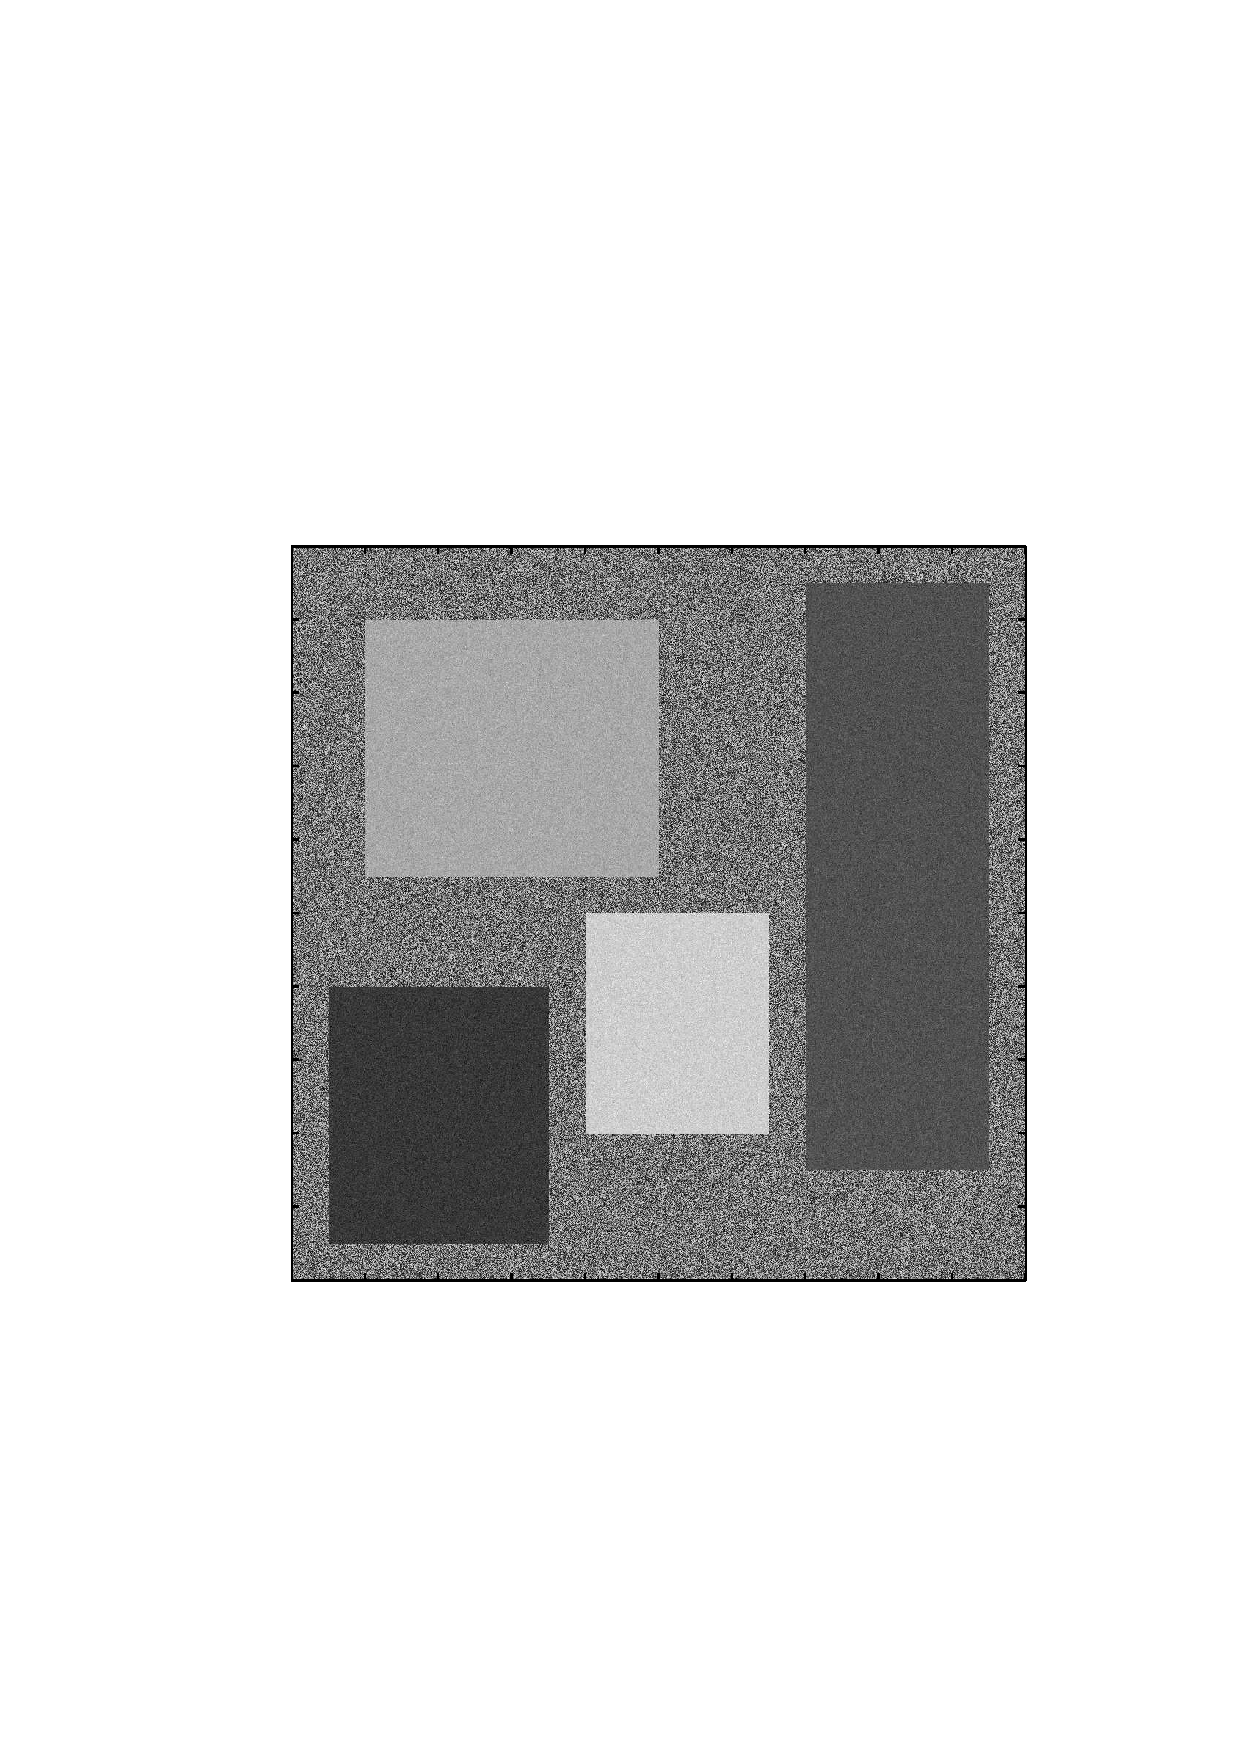
\includegraphics[width=45mm]{O2}&
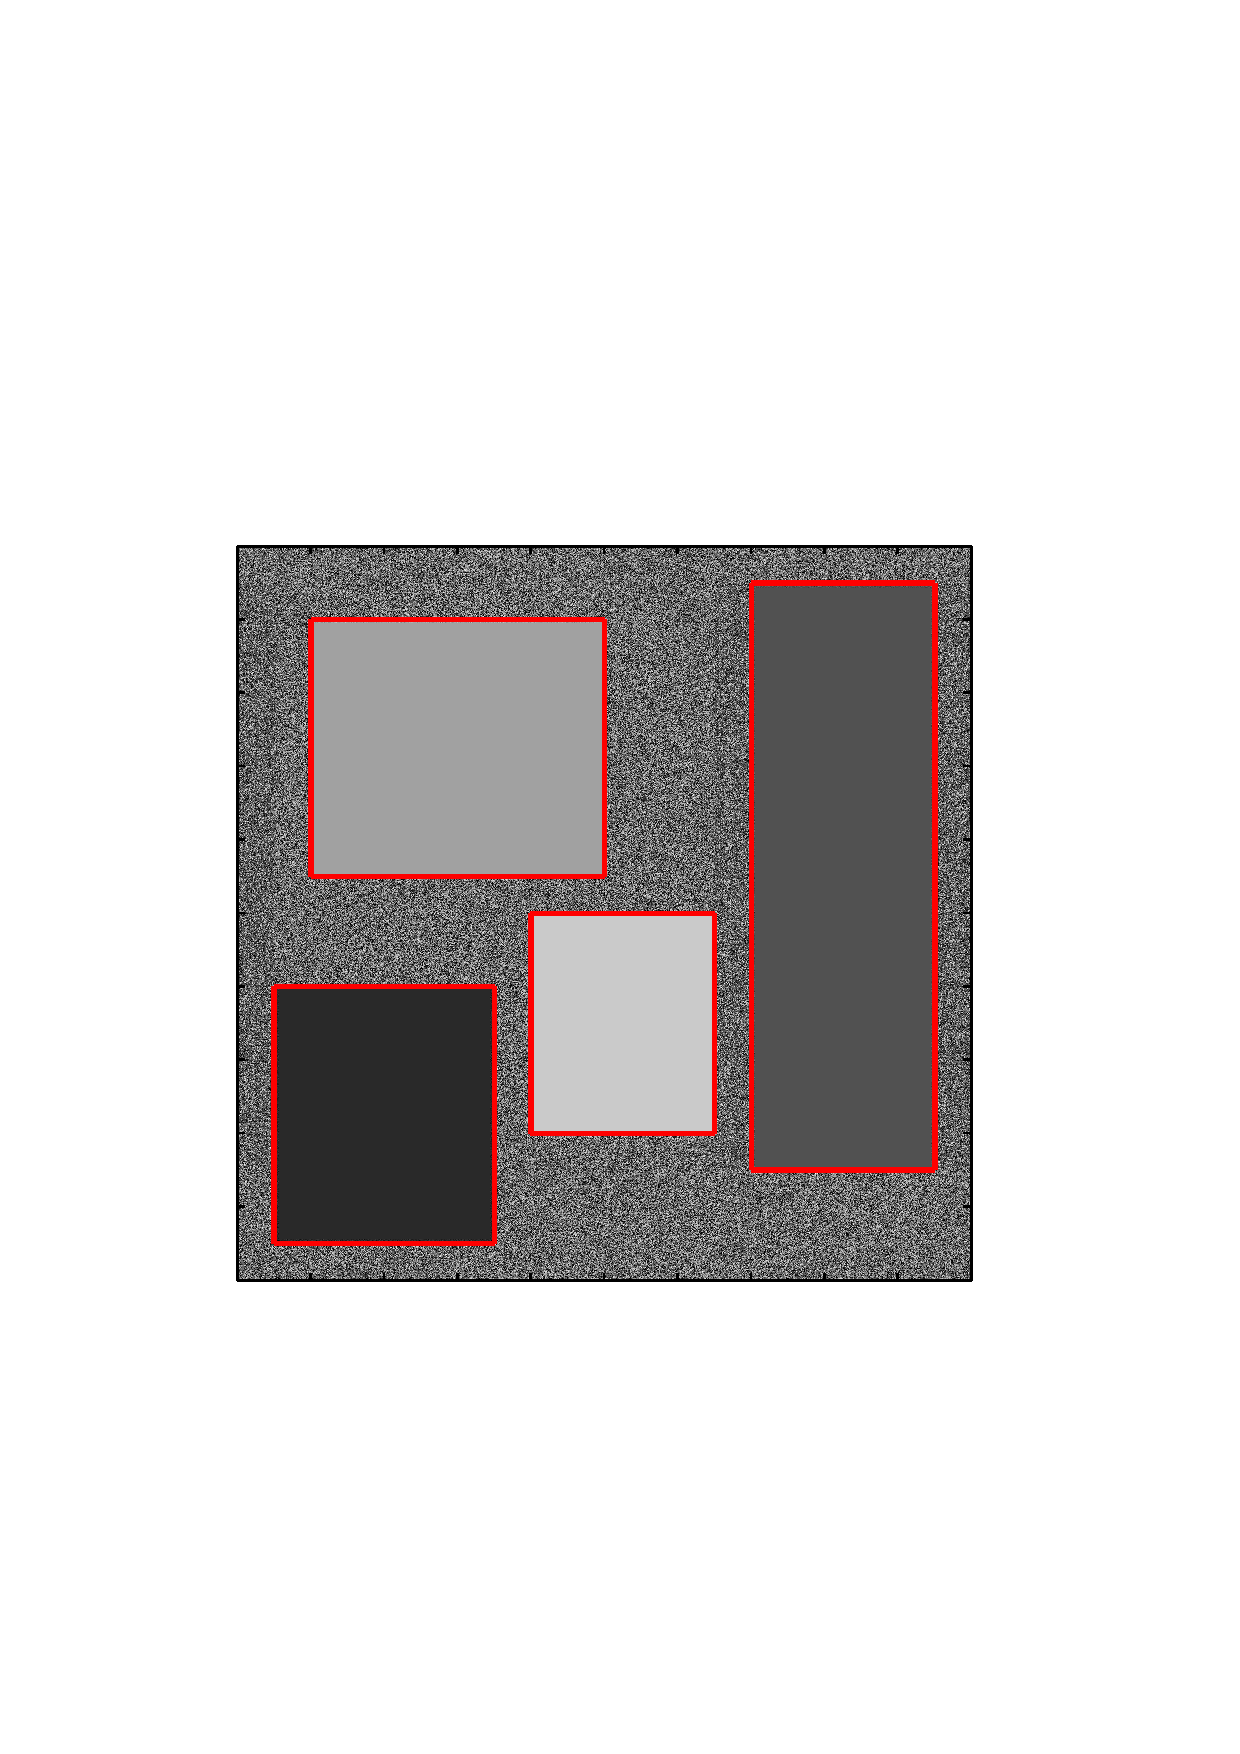
\includegraphics[width=45mm]{syn2R}&
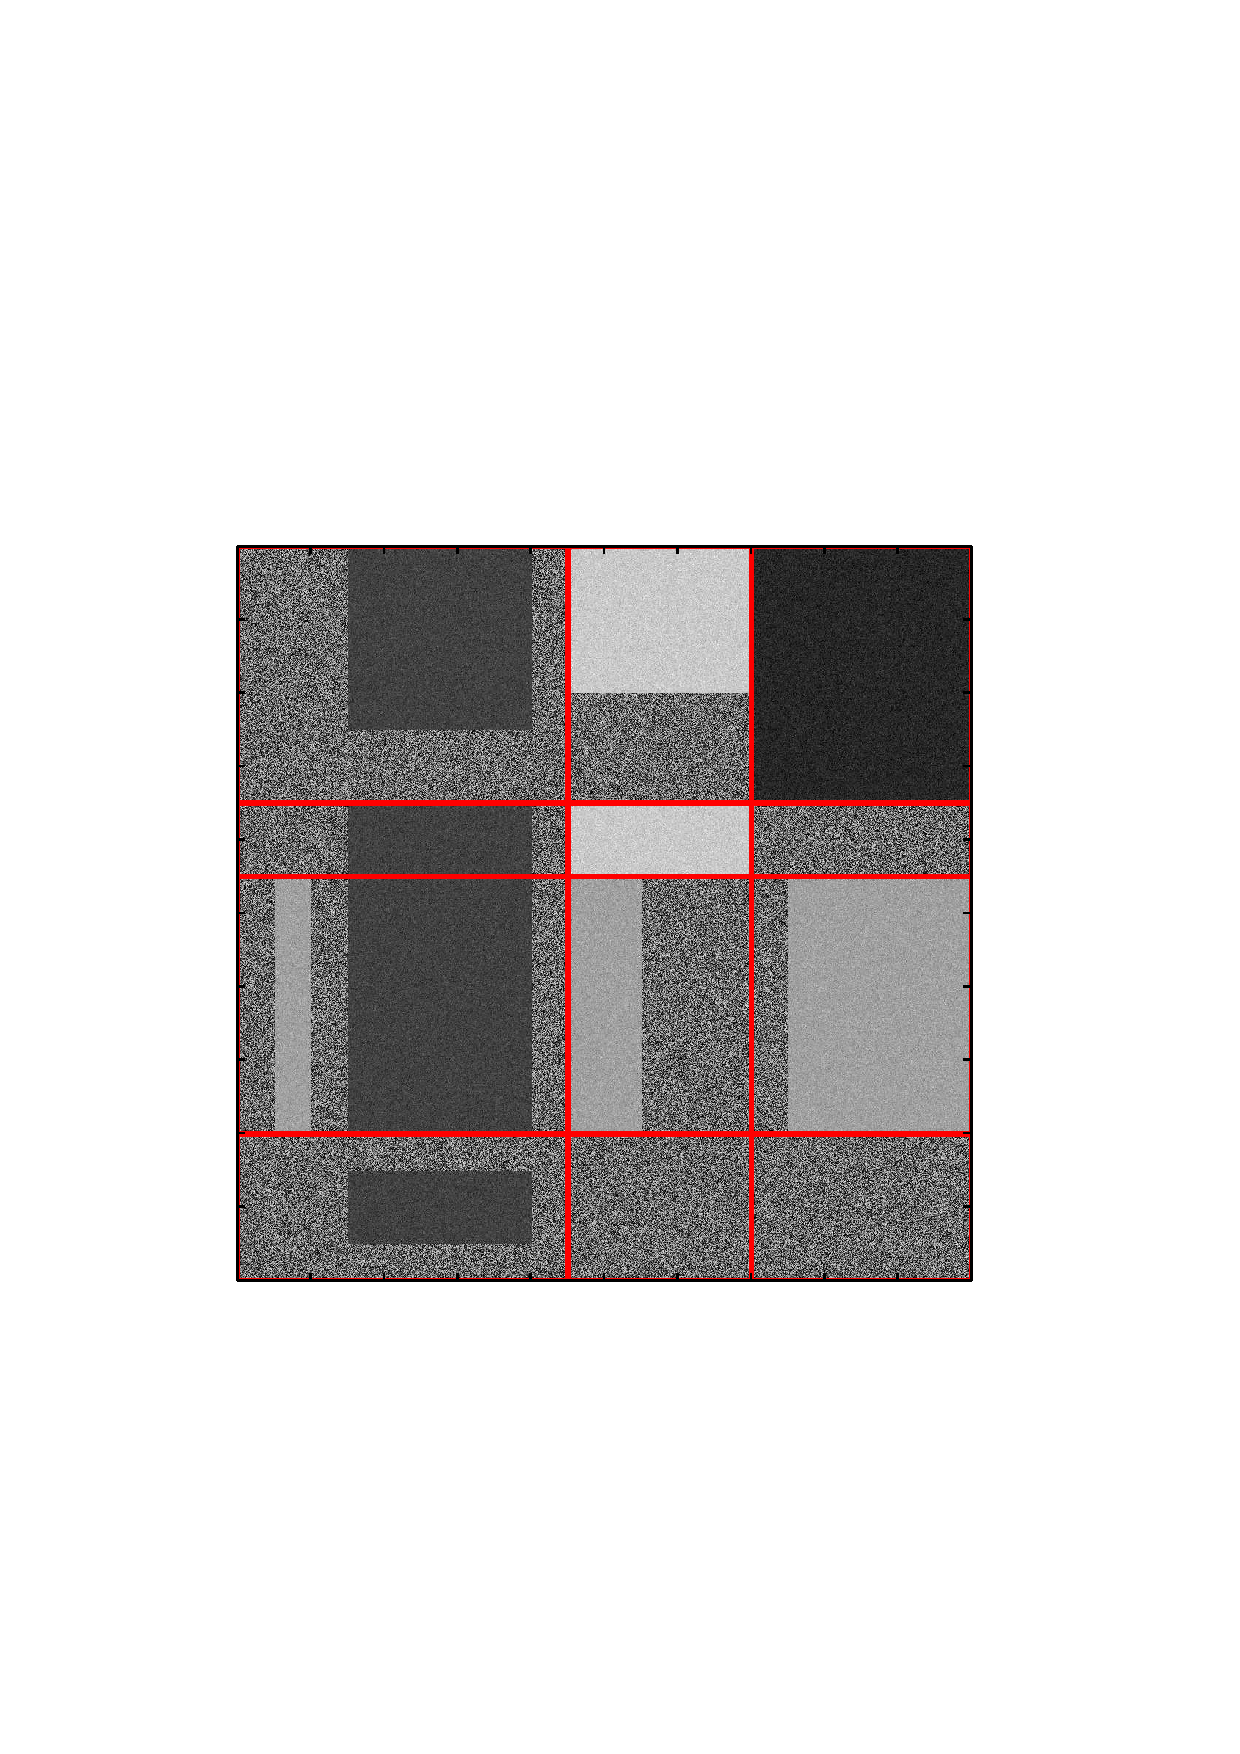
\includegraphics[width=45mm]{inf2}\\
(g) 随机分布矩阵  & (h) CoSync &  (i) ITCC\\
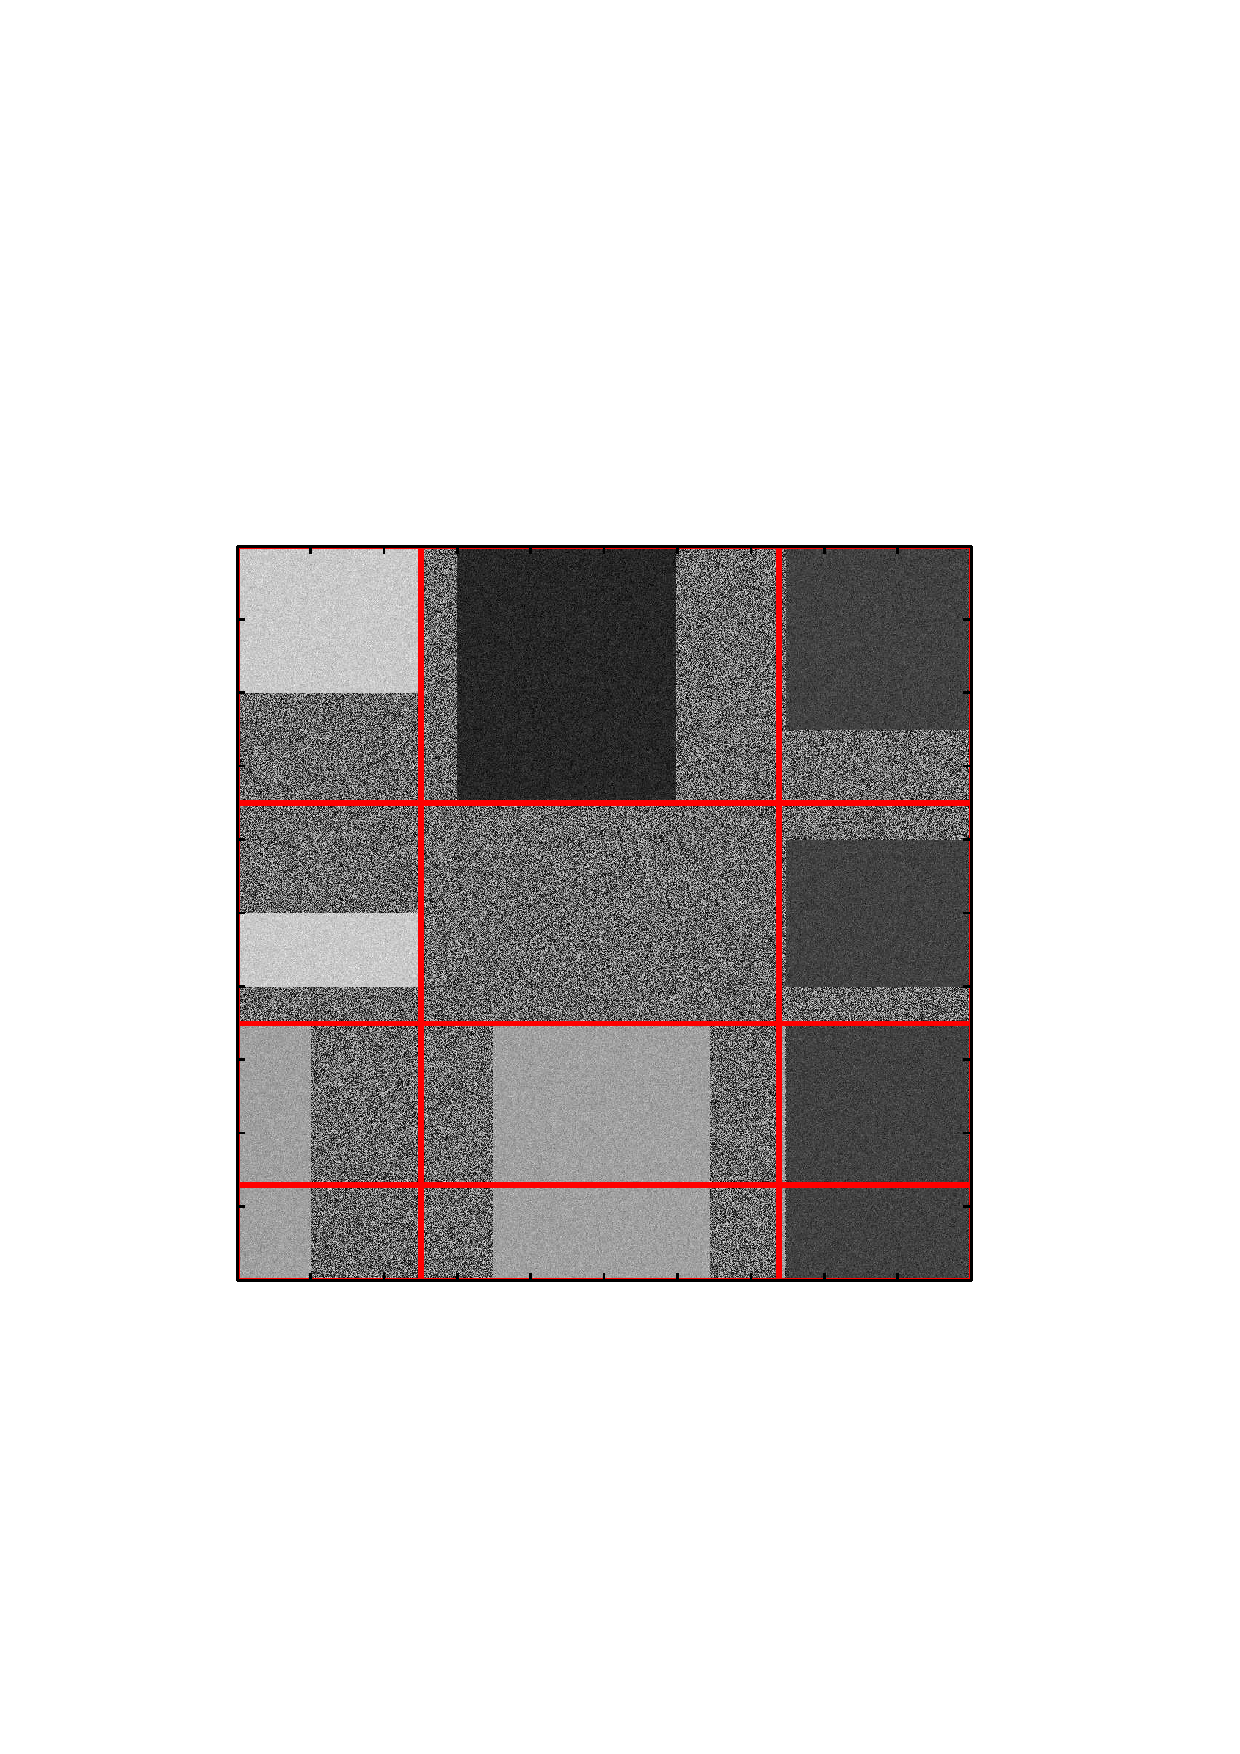
\includegraphics[width=45mm]{residue2}&
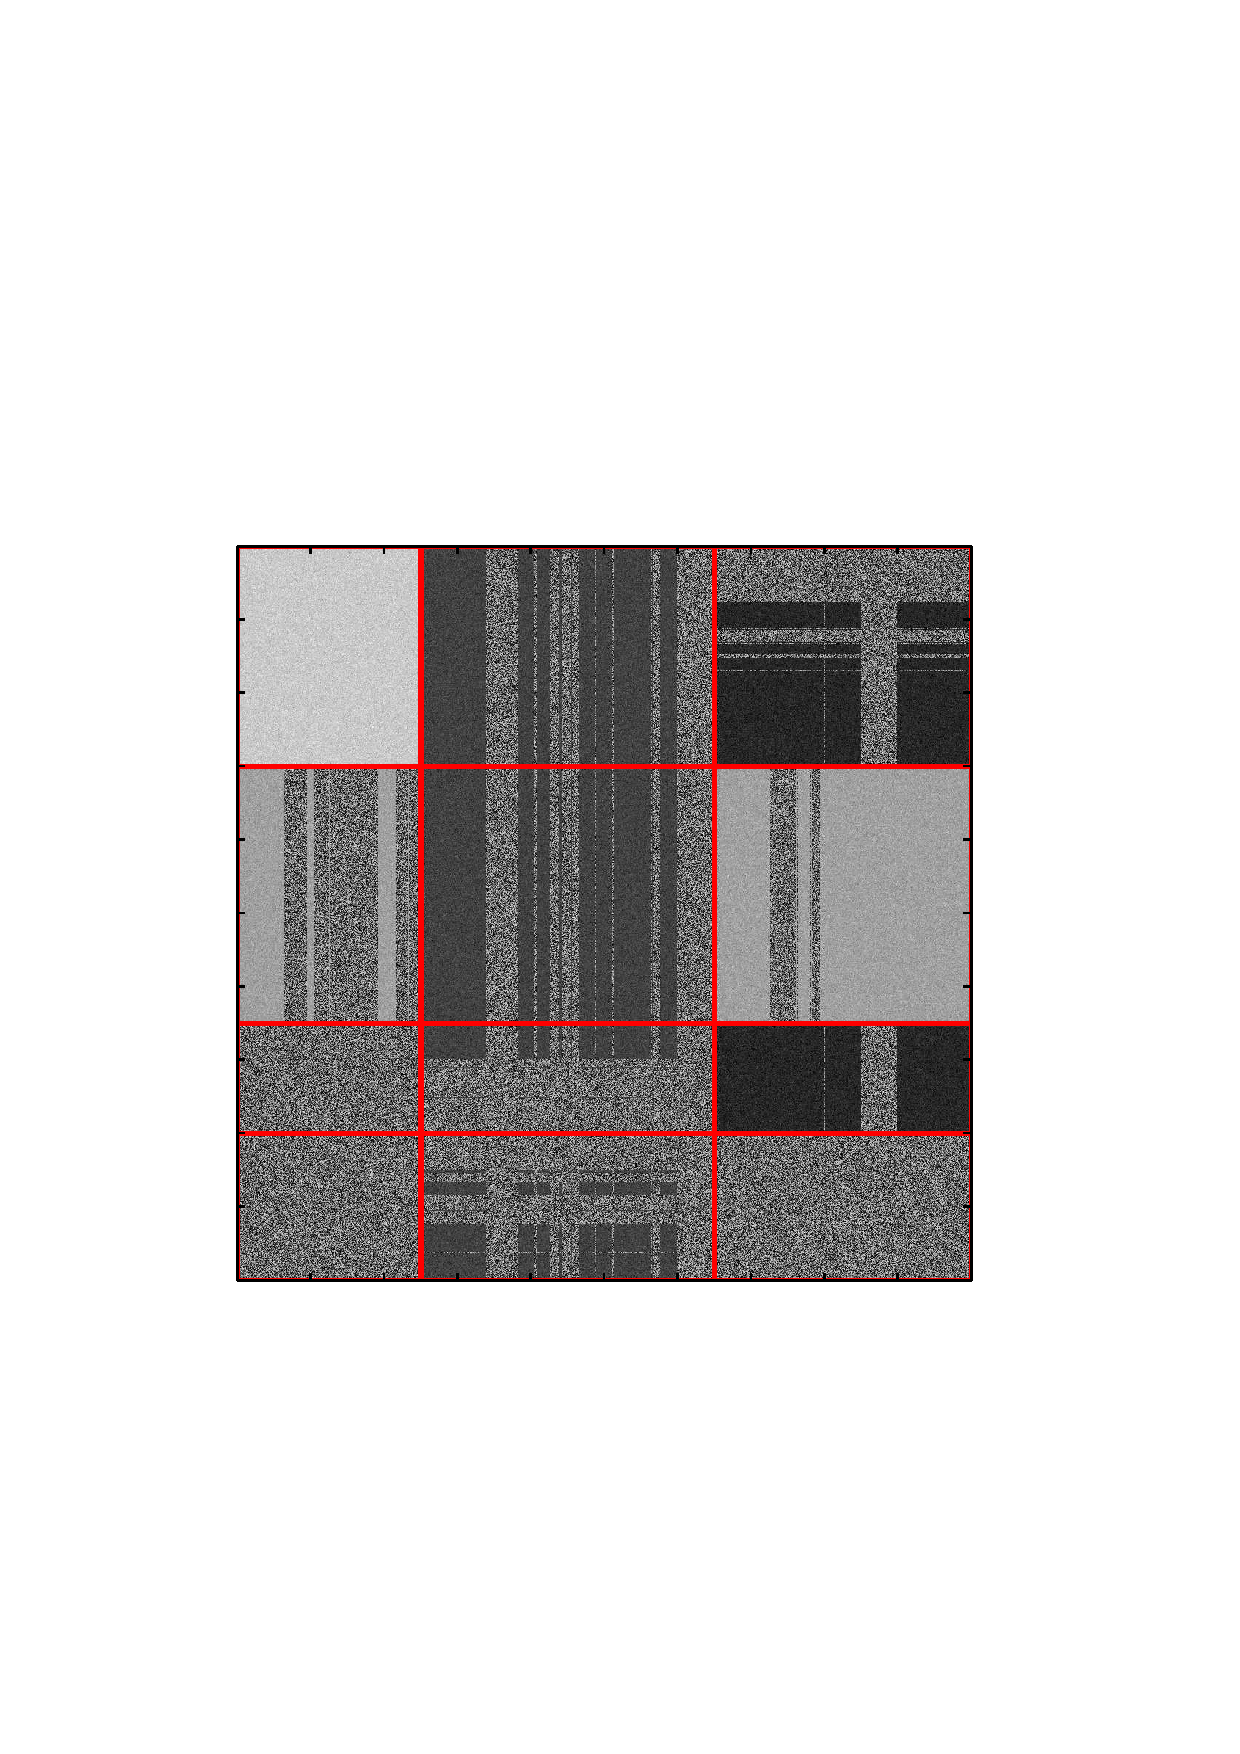
\includegraphics[width=45mm]{spectral2}&
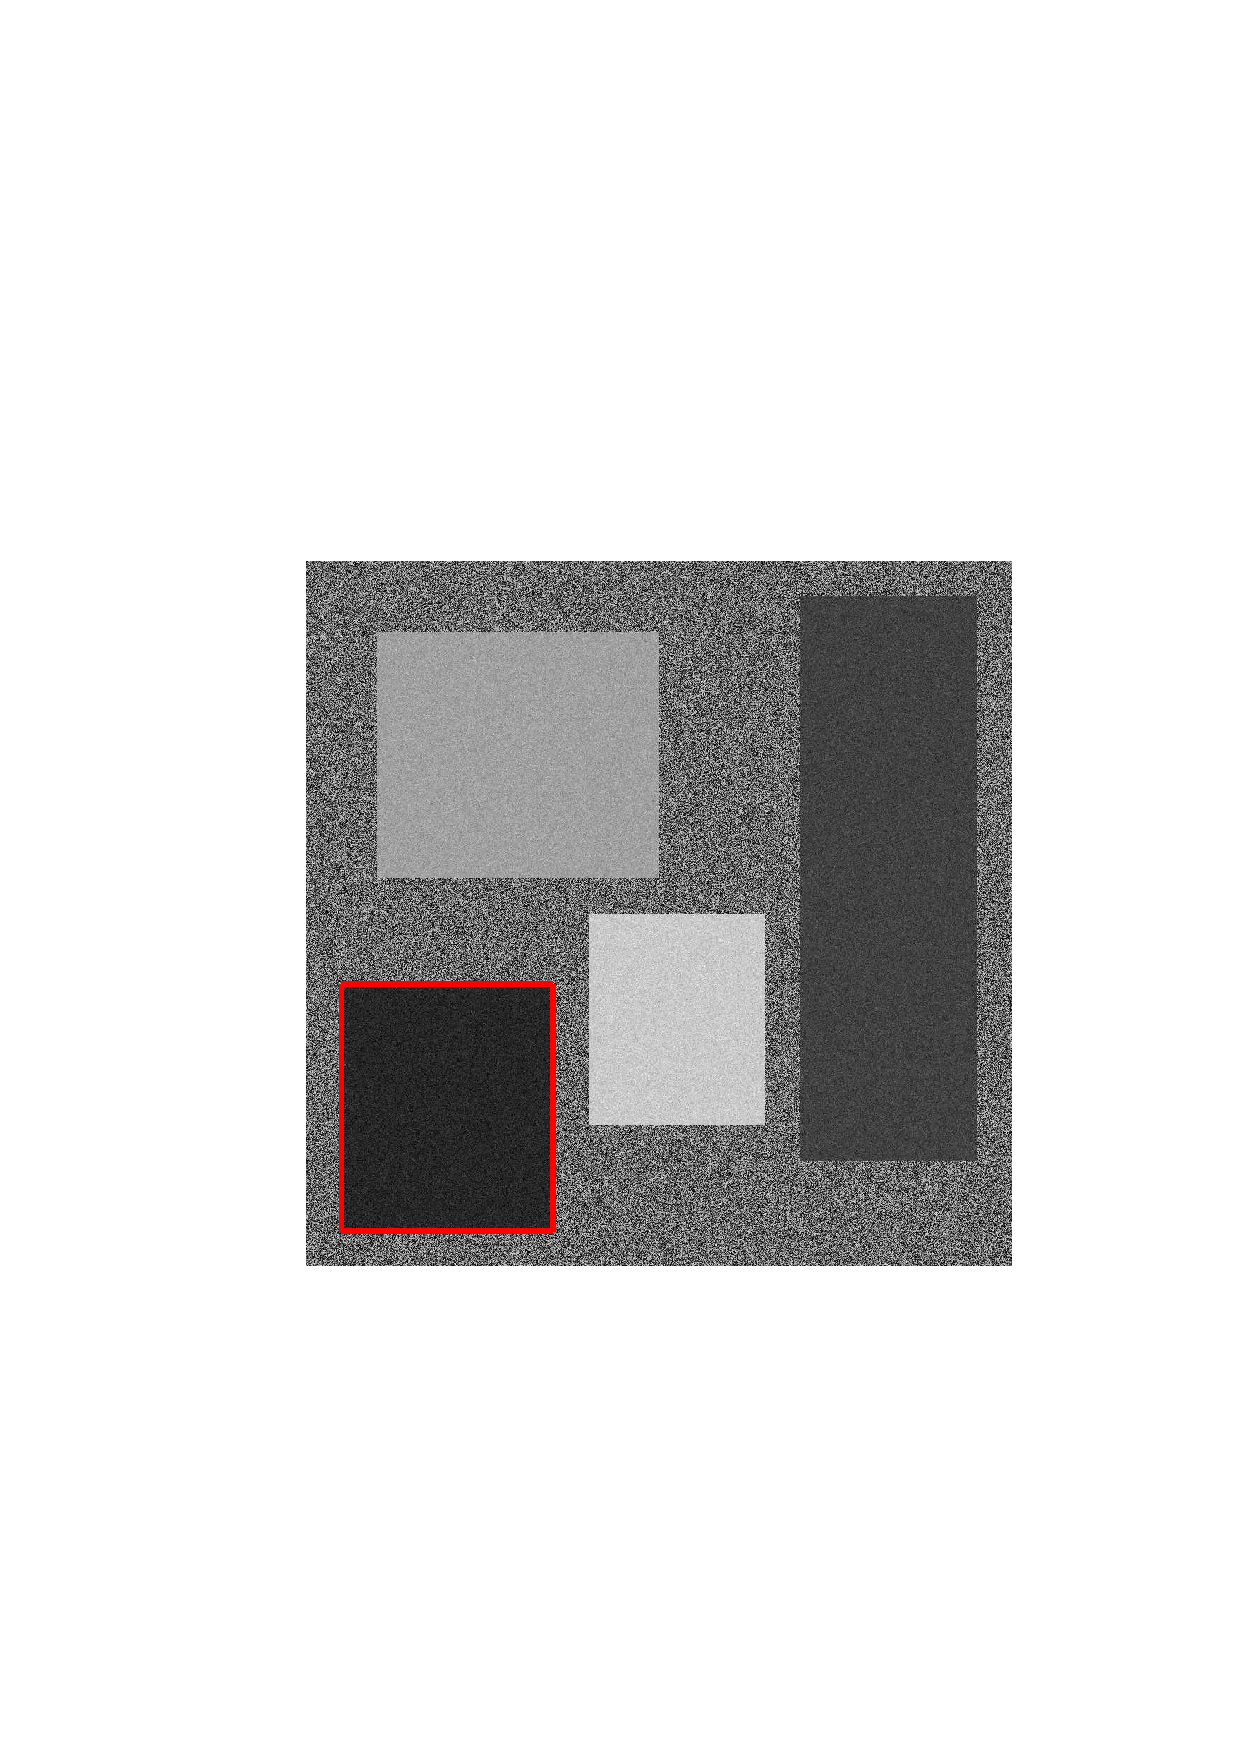
\includegraphics[width=45mm]{plaid2}\\
(j) MSSRCC &  (k)  Spectral &  (l) Plaid
\end{tabular}
\caption{五种算法在棋盘分布矩阵和随机分布矩阵上运行结果图。(a)为棋盘分布原矩阵。(b)-(f)为五种算法在棋盘分布矩阵上的聚类结果可视化。(g)为随机分布原矩阵。(h)-(l)是五种算法在随机分布矩阵上的聚类结果可视化。
图中红色方框为算法找出的聚类簇。}
\label{fig:yiqi_r}
\end{figure*}
% \pagenumbering{}



\section{基因表达数据上的算法实现及评估}
% \pagenumbering{arabic}
% \setcounter{page}{28}
\label{sec:gene}
在本小节中,我们将在基因数据集上对\cosync算法进行测试。首先我们将介绍选本次实验选用的基因数据集,之后给出\cosync运行的聚类簇可视化结果,最后根据生物信息学中对基因的评价方法来说明\cosync算法的运行结果。

\subsection{基因数据集选取}
DNA微阵列数据是一种观测基因在特定样本上表达程度的数据\footnote{\url{https://en.wikipedia.org/wiki/DNA_microarray}},可以用一个矩阵来表示,其中行代表基因,列代表特定样本,如不同个体,不同组织,或者不同环境下观测到的数据。

本文第一章提过,双边聚类这一领域就是在基因数据集上发展起来的,后面只有少部分方法能扩展到购物篮数据集以及文本-词汇数据集上。导致这一现象的原因是现实情况中,只有基因数据集密集无缺失值,这是距离度量的必要条件。

在本章第\ref{subsec:principle}节中的数据集选取原则中提到,\cosync可以处理的数据集必须是数值型无缺失值的,基因数据集满足这一条件。然而基因数据集的尺寸规模几乎都为$1000\times10$量级,即数千规模的基因在数十个样本上的表达程度,使得矩阵的行列比例严重失调。前文说过,数据集比例失调可能会带来算法正确率降低。面对这一困扰,我们只能在实验中尽量以调参数的方式来进行应对。

本次实验中,我们选取了四个通用的基因表达数据集\footnote{基因数据集矩阵及对应的基因名称来源:\url{http://datam.i2r.a-star.edu.sg/datasets/krbd/index.html}},皆被国际众多知名双边聚类算法所使用,其信息总结如表\ref{tab:dataset}。
\vspace{3mm}
\tabcolsep=5pt
\begin{table}[!htb]\renewcommand{\arraystretch}{1.3}
\center \caption{四个基因数据集的统计信息表}
\small
\begin{tabular}{ccccc}
\hlinew{1pt}
\textbf{数据集}& \#\textbf{基因数目}& \#\textbf{样本数目} & \textbf{样本类别名称}&  \textbf{样本分布}\\
\hlinew{1pt}
Colon  &  1096 & 62 &Normal/Tumor& 20/42  \\
Leukemia   & 3571 & 72 &ALL/AML & 47/25    \\
Lung    & 2401 & 181 &ADCA/MPM& 150/31 \\
MLL & 2474 & 72  & ALL/AML/MLL&24/28/20 \\ \hlinew{1pt}
\end{tabular}
\label{tab:dataset}
\end{table}

可见数据集的行列比例很不均衡。其样本类别只有两个或者三个,其中ALL、AML、ADCA、MPM和MLL均为疾病名称的缩写,而基因没有直接的类别标签。
%其结果评价将用\ref{subsec:analysis}中所述的基因集丰富度分析来进行。

\subsection{\cosync在基因数据集上的联合簇挖掘}
真实数据集与人工数据集的差别在于真实数据集的联合簇数目更多、大小更不规律、分布更不均衡,取不同的$\epsilon$邻域邻居将得到不同层次下的联合簇。我们结合专家知识来制定合适的$\epsilon$取值范围,在取值范围内用\cosync对上述数据集进行多次测试后,得到一些特定值的大尺寸联合簇。

我们将\cosync,ITCC,MSSRCC,Spectral Clustering和Plaid算法在四个数据集上进行了实验。如前文所述,基因空间的评价无法直接对比,其将用\ref{subsec:analysis}中所述的基因集丰富度分析来来进行。故我们仅将对他们找出的联合簇中的样本空间进行评价对比,用\ref{subsec:evaluation}节中叙述的准确率和召回率作为评价指标。表\ref{tab:compare}展示了四种算法在四个数据集上找到的所有联合簇在样本空间中的评价。

\vspace{2mm}
\tabcolsep=3pt
\begin{table}[!htb]\renewcommand{\arraystretch}{1.2}
\center \caption{五种算法在四个数据集上找出聚类簇的样本空间评价}
\small
\begin{tabular}{c|ccc|ccc|cc|cc|cc}
\hlinew{1pt}
\multirow{2}{*}{\textbf{}} & \multicolumn{3}{c|}{\textbf{ CoSync}}&\multicolumn{3}{c|}{\textbf{Plaid}}& \multicolumn{2}{c|}{\textbf{ ITCC}} &\multicolumn{2}{c|}{\textbf{ MSSRCC}} & \multicolumn{2}{c}{\textbf{ Spectral}}  \\
\cline{2-13}
  & \#C &Pre. & Rec. & \#C &Pre. & Rec. & \#C & Avg. &\#C & Avg. &\#C & Avg. \\[0.4ex] \hlinew{1pt}
Colon & 11& 0.95 & 0.66& 4&0.71&0.66& 2& 0.82& 2& 0.86 &2 & 0.73\\
Leukemia & 28& 0.96 & 0.71 &2&0.81&0.43& 2& 0.95&2 & 0.93&2 & 0.74\\
Lung& 23& 1.00& 0.96 &3&1.00&0.50& 2& 0.85& 2& 0.99& 2& 1.00 \\
MLL& 23& 0.99 & 0.67 &4&0.88&0.88&3 &0.83 &3 &0.93 &3 &0.64 \\ \hlinew{1pt}
\end{tabular}
\label{tab:compare}
\end{table}

可以看到ITCC,MSSRCC和Spectral Clustering算法的由于基于划分,故其样本空间划分数目已经提前被指定好,均为数据中样本类别的真实数目。在自动找寻联合簇的算法\cosync和Plaid当中,Plaid找出的簇仅为$2\sim4$个,而\cosync算法在Colon数据集中找出11个联合簇,而其他三个数据集上,都发掘出了$20$个以上的联合簇。

关于样本的评价标准,\cosync在四个数据集上准确率都达到了令人满意的$95\%$\\以上,而召回率达到了$66\%$以上。这说明了\cosync算法找出的联合簇都能代表真实数据中的数据结构。而召回率在这重要性不是很高,因为这仅代表着算法找出的样本没有覆盖整个样本维空间。从准确率上来看,其他算法的性能都没有超过\cosync,而从召回率的角度看,基于划分的方法明显超出\cosync算法,这是合理的结果。

其次,我们还能从图中看出,数据集Lung在五个算法下都表现出了优良的性能,而Colon数据集在5个算法下的性能都不如其他数据集。这说明数据集本身的结构会影响所有的算法效能。

为了观察\cosync找出的聚类簇的具体形态,我们为上述结果中\cosync的前十大尺寸的聚类簇进行更细的观察。表\ref{tab:real}列举了四个数据集中尺寸最大的10个联合簇的信息,包括该联合簇的行、列数目,以及关于样本维度上的精确率和召回率。




从表中的结果中我们可以看出来,\cosync的找寻质量还是较高的。大多数聚类簇的准确率都是$1.00$,在Lung数据集上甚至所有的聚类簇在样本维空间上的聚类准确率都为$1.00$。这一结果更肯定了我们上述的判断:\cosync算法找出的聚类簇的准确率很高。

ITCC,MSSRCC和Spectral Clustering算法这样基于划分的方法在没有标签的情况下, 决定划分簇数目是非常困难的,错误的参数指定将会带来完全偏离真实情况的结果。接下来,我们将对五种算法找出的联合簇对基因维度进行评价。

\subsection{基因集丰富度分析}
\label{subsec:analysis}
我们实验数据的基因表达数据来源于对数以千的基因在特定样本下进行表达的探测。这其中样本的分类是明确的,但是基因却没有确定的类标签。为了衡量数据挖掘、人工智能算法对基因分类、聚类的结果,一种专门的衡量指标被提了出来,即基因集丰富度分析。

基因丰富度分析\footnote{\url{https://en.wikipedia.org/wiki/Gene_set_enrichment}},也称为功能性丰富度分析,是一种为基因和蛋白质的归类显著性进行评判的一种分析方法。基因没有类标签,但大量的实验表明在一些特定的试验下,观测基因经历一些生物过程最终表达为蛋白质的情况,一部分基因会表达得更明显,而另外的基因则被抑制或不表达。搜集这些历史记录,大量的特定的基因集合被记录下来,它们被记录在基因本体库\footnote{\url{https://en.wikipedia.org/wiki/Gene_ontology}}中。基因本体库中的特定基因集合可以分为以下三个邻域类别:
\begin{itemize}
\item \textbf{~~细胞组件(cellular component)}:细胞的每个部分和细胞外环境。
\item \textbf{~~分子功能(molecular function)}:基因产物在分子级别的主要活动,比如结合以及催化。
\item \textbf{~~生物过程(biological process)}:细胞内发生的,可以定义开始和结束的事件或行动。
\end{itemize}

有了基因本体库,我们用算法对基因进行聚类的结果便有了比对的参照物。针对我们算法找出的基因数据集与基因本体中不同情况下的基因集合,用假设假设检验\footnote{\url{https://en.wikipedia.org/wiki/Statistical_hypothesis_testing}}的方式,便能得知我们找出的基因集合是否合理:是否完全属于某一个基因本体中的基因集合?是否太过随机,没有任何代表性?用这种方式,我们便能评价\cosync找出的聚类簇中基因空间中的结果好坏。

\tabcolsep=4pt
\begin{table*}[!h]\renewcommand{\arraystretch}{1.2}
\center \caption{各个数据集上前十大联合簇信息。其中 $P$ 和 $R$ 分别代表每个联合簇在样本空间中的精确率和召回率。 $No.G.$ 和 $No.S.$分别是联合簇包含的基因和样本的数目。 $N$ 和 $T$ 分别代表Colon数据集中的Normal和Tumor。 $A$ 和 $M$ 分别代表Lung数据集中的ADCA和MPM。 $AL$, $AM$ 和 $ML$ 分别代表Leukemia和MLL数据集中的ALL,AML和MLL。}
\small
\begin{tabular}{ccccccccccccc}
\hlinew{1pt}
&~~&\multicolumn{5}{c}{\textbf{Colon}} & &\multicolumn{5}{c}{\textbf{Leukemia}} \\ \cline{3-7} \cline{9-13}
 \textbf{cID} &~~& \textbf{Size}   &\textbf{No.G. }& \textbf{No.S. } & \textbf{P} &\textbf{R}&~~& \textbf{Size}   &\textbf{No.G.} & \textbf{No.S.}  & \textbf{P} &\textbf{R}\\
\hlinew{1pt}
1   &~~& 1480  &296   & 5(N)   &1.00  & 0.23 &~~&3216 & 268 & 12(7AL/5AM) &0.58  &  0.15  \\
2   &~~& 966   &138   &7(5N/2T)&0.71  & 0.23 &~~&2570 &514  & 5(4AM/1AL)  &0.80  &0.16    \\
3   &~~& 666   &111   &6(T)    &1.00  &0.15  &~~&2320 &464  & 5(AL)        &1.00  &0.11   \\
4   &~~& 510   &85    &6(5N/1T)&0.83  &0.23  &~~&1480 &296  & 5(AL)        &1.00  &0.11   \\
5   &~~& 420   &84    &5(N)    &1.00  &0.13  &~~&1215 &243  & 5(AM)        &1.00  &0.20   \\
6   &~~& 290   &58    &5(T)    &1.00  &0.13  &~~&625  &125  & 5(AL)        & 1.00 &  0.11 \\
7   &~~& 205   &41    &5(T)    &1.00  &0.13  &~~&320  &64   &5(AL)         &1.00  &0.11   \\
8   &~~& 125   &25    &5(T)    &1.00  &0.13  &~~&294  &49   &6(AM)         & 1.00 &0.24   \\
9   &~~& 65    &13    &5(T)    &1.00  &0.13  &~~&264  &22   &12(AL)        &1.00  &0.26   \\
10  &~~& 49    &7     &7(T)    &1.00  &0.13  &~~&242  &22   &11(AL)        & 1.00 &  0.23 \\
\hlinew{1pt}


&~~&\multicolumn{5}{c}{\textbf{Lung}} & &\multicolumn{5}{c}{\textbf{MLL}}\\ \cline{3-7} \cline{9-13}
 \textbf{cID} &~~&  \textbf{Size}   &\textbf{No.G.} & \textbf{No.S.}   & \textbf{P}&\textbf{R}&~~&  \textbf{Size}   &\textbf{No.G.} & \textbf{No.S.}   & \textbf{P }&\textbf{R}\\
 \hlinew{1pt}
1  &~~& 5614   & 401  & 14(A)   & 1.00  & 0.09 &~~&4228   & 302  & 14(AM)   & 1.00      & 0.50  \\
2  &~~& 4394   & 338  & 13(M)   & 1.00  & 0.42 &~~&3765   & 251  & 15(AL)   & 1.00      & 0.63  \\
3  &~~& 3960   & 264  & 15(A)   & 1.00  & 0.10 &~~&2954   & 211  & 14(AL)   & 1.00      & 0.58  \\
4  &~~& 3806   & 346  & 11(M)   & 1.00  & 0.36 &~~&2071   & 109  & 19(AM)   & 1.00      & 0.68   \\
5  &~~& 2344   & 293  & 8(A)    & 1.00  & 0.05 &~~&1584   & 99   & 16(AM)   & 1.00      & 0.57  \\
6  &~~& 2210   & 221  & 10(M)   & 1.00  & 0.32 &~~&918    & 102  & 9(AL)   & 1.00      & 0.38   \\
7  &~~& 1770   & 177  & 10(M)   & 1.00  & 0.32 &~~&890    & 89   & 10(AL)   & 1.00      & 0.42   \\
8  &~~& 1035   & 115  & 9(M)    & 1.00  & 0.29 &~~&715    & 143  & 5(3ML/2AL) & 0.60  & 0.15   \\
9  &~~& 950    & 190  & 5(A)    & 1.00  & 0.03 &~~&533    & 41   & 13(AM)   & 1.00      & 0.46   \\
10 &~~& 420    & 30   & 14(M)   & 1.00  & 0.45 &~~&510    & 34   & 15(AM)   & 1.00      & 0.54   \\

\hlinew{1pt}

\end{tabular}
\label{tab:real}
\end{table*}

统计假设检验用p-value\footnote{\url{https://en.wikipedia.org/wiki/P-value}}来作为显著与否的评价指标。其概念定义如下:

\textbf{显著性因子p-value}:一种在原假设为真的前提下出现观察样本以及更极端情况的概率。设某假设为$H_0$,则p-value在$H_0$为真的条件下,因样本偏差太大而拒绝$H_0$的概率,即:
\begin{equation*}
p-value = P(\text{拒绝接受}H_0\big{|}H_0\text{为真})
\end{equation*}

p-value值越小,则说明拒绝$H_0$的概率越小,也就是假设$H_0$越可信。当p-value\\取$0$时候,假设$H_0$与观测相比毫无差别。而当p-value值打过一定程度时候,结果就不可信了。对此人们通常设置一个阈值$\alpha$,当$p-value\ge\alpha$时,便拒绝假设$H_0$。

\vspace{2mm}
在基因库丰富度分析中,令真实的一个基因集合为$\mathcal{G}$,而预测出来的基因集合为$\hat{\mathcal{G}}$,对应假设$H_0$的命题为:
\begin{equation*}
H_0 = \{\hat{\mathcal{G}}\subseteq{}\mathcal{G}\}
\end{equation*}

即p-value在基因库丰富度分析中,可以作为任意给定的基因集合的显著性的指标。由此我们可以预先设置一个拒绝阈值:$\alpha$,之后对每一个聚类簇的基因与基因本体中每一个基因集合对比,算出一个对应的p-value值,若其大于$\alpha$,则不考虑基因本体中这个基因库。最后我们对基因本体库中的满足$p-value\leq\alpha$的基因集合列举出来。我们的算法找出的基因簇很可能就是这些基因集的子集。

值得说明的是,给定我们的基因集合,对基因本体库里任意的基因集合都能算出一个p-value,虽然这些p-value本身值越小越好,但它们互相之间是不可比较的。例如我们不能因为我们的基因集对与艾滋病蛋白相关的基因本体集的p-value比其于白血病蛋白相关的基因本体集的p-value值小,就说明我们的基因集更倾向于与艾滋病的蛋白表达相关。也正是这个原因,有三个浅显的结论:
\begin{itemize}
\item ~~不同算法间找出聚类簇中基因集合的p-value值之间不能相互比较。
\item ~~同一算法中,不同聚类簇基因集的p-value值不能相互比较。
\item ~~同一算法中,同一聚类簇中的基因集对基因本体中不同基因集的p-value值之间不能相互比较。
\end{itemize}

由于\cosync与其他算法找出聚类簇的基因集显著结果无法比较,故本文中我们仅对我们的\cosync算法进行基因集丰富度分析。事实上,现在已有用于基因库丰富度分析的公开网站,并且已经很成熟和快速,本次我们将使用基因本体库最齐全的Gene Ontology Consortium网站(\url{http://geneontology.org/})来进行丰富度分析。表\ref{tab:annotations}列出了\cosync联合簇找出的联合簇基因集进行丰富度分析的结果,阈值$\alpha$取为$0.05$。受于篇幅的限制,此处仅列出每个数据集中前3大的联合簇的分析结果。

表中CC和BP以及后面跟的专业名词分别代表细胞组件与生物过程中特定的物质组成部分或者生物学过程。可以看出每个聚类簇在与基因本体库中的基因集进行匹配时,p-value$\le0.05$的基因集最少在Colon数据集中能匹配到65个,最多在Leukemia数据集中能匹配539个。找出其各自p-value最小的4个进行进一步剖析,可以看到它们的p-value都小于$1\times10^{-3}$级别。有理由相信这部分基因就是对应细胞组件或者生物过程中某特定过程的组成基因的子集。图\ref{cocluster}中,我们对每个数据集中大尺寸联合簇进行了可视化,由于篇幅原因,对于样本的每个类别我们只取一个聚类簇。

\vspace{2mm}
\pic[!htb]{基因表达数据联合簇可视化图}{width=120mm}{cocluster}

从上面简单的评估中,我们可以看出\cosync能够找到一些高质量的聚类簇。关于对聚类基因集的更进一步权威的生物学验证,已经超出本实验的范围,本文不再展开。

\tabcolsep=1pt
\begin{table*}[!htb]\renewcommand{\arraystretch}{0.9}
\center \caption{\cosync算法找出的联合簇在基因空间上丰富度分析结果表。这里 BP 代表 “Biological Process”,CC 代表 “Cellular Component”。 \#Annotations 代表 p-value $<$0.05的所有基因本体库中的基因集数目。}
\scriptsize
\begin{tabular}{c|c|cclccc}
\hlinew{0.85pt}\textbf{Data Sets} &\textbf{ CluID} & \#\textbf{Genes} & \#\textbf{Annotations}&\textbf{Top Enriched Annotations} &\textbf{Count} & \textbf{Percentage (\%) } & \textbf{P-Value}  \\[0.4ex] \hlinew{0.85pt}

%Colon
\multirow{12}{*}{Colon} &\multirow{4}{*}{C1}& \multirow{4}{*}{296} &\multirow{4}{*}{214}& CC:cytosol                &34  & 23.61\%   & 5.84E-07\\
&&&&CC:plasma membrane part    &42  & 29.17\%    &3.01E-05\\
&&&&BP:negative regulation of molecular function          &13  &9.03\%     &7.69E-05\\
&&&& BP:striated muscle tissue development          &8  &5.56\%     &1.34E-04\\
\cline{2-8}
 &\multirow{4}{*}{C2}& \multirow{4}{*}{138} &\multirow{4}{*}{157}& CC:plasma membrane part & 22 &37.29\%& 4.81E-05\\
&&&& CC:plasma membrane& 28 &47.46\%&3.87E-04\\
&&&& CC:cytosol &15&25.42\%&5.20E-04\\
&&&& CC:actin cytoskeleton &7 & 11.86 \%&6.69E-04\\  \cline{2-8}
 &\multirow{4}{*}{C3}& \multirow{4}{*}{111} &\multirow{4}{*}{65}& BP:regulation of system process & 8 &15.69\%& 7.55E-05\\
&&&& BP:heart development & 6 & 11.76\% &7.81E-04\\
&&&& BP:negative regulation of molecular function& 7 & 13.73\%& 8.82E-04\\
&&&& CC:striated muscle thin filament & 3 &5.88\% & 1.13E-03 \\
\hline
%Leukemia
\multirow{12}{*}{Leukemia} &\multirow{4}{*}{C1}& \multirow{4}{*}{268} &\multirow{4}{*}{300}
&BP:response to endogenous stimulus & 27 & 10.67\% & 2.47E-09\\
&&&&CC:plasma membrane part & 71 & 28.06\% & 4.54E-09\\
&&&&CC:integral to plasma membrane & 48 & 18.97\% & 5.34E-09\\
&&&&BP:response to hormone stimulus & 25 & 9.88\% & 7.40E-09\\
\cline{2-8}
&\multirow{4}{*}{C2}& \multirow{4}{*}{514} &\multirow{4}{*}{415}
&CC:cytosol & 123 & 24.45\% & 2.08E-28\\
&&&&CC:intracellular organelle lumen & 142 & 28.23\% & 1.10E-26\\
&&&&CC:organelle lumen & 142 & 28.23\% & 1.13E-25\\
&&&&CC:membrane-enclosed lumen & 142 & 28.23\% & 8.10E-25\\
\cline{2-8}
&\multirow{4}{*}{C2}& \multirow{4}{*}{464} &\multirow{4}{*}{539}
&CC:plasma membrane part & 114 & 25.79\% & 2.37E-11\\
&&&&CC:integral to plasma membrane & 73 & 16.52\% & 2.72E-10\\
&&&&CC:intrinsic to plasma membrane & 74 & 16.74\% & 2.95E-10\\
&&&&CC:plasma membrane & 160 & 36.20\% & 2.30E-09\\
\hline
% %Lung
\multirow{12}{*}{Lung} &\multirow{4}{*}{C1}& \multirow{4}{*}{401} &\multirow{4}{*}{308}
&CC:cytosol & 88 & 23.34\% & 4.71E-17\\
&&&&CC:intracellular organelle lumen & 87 & 23.08\% & 2.18E-09\\
&&&&CC:organelle lumen & 88 & 23.34\% & 2.96E-09\\
&&&&CC:membrane-enclosed lumen & 89 & 23.61\% & 3.47E-09\\
\cline{2-8}
&\multirow{4}{*}{C2}& \multirow{4}{*}{338} &\multirow{4}{*}{183}
&CC:cytosol & 62 & 19.68\% & 1.74E-09\\
&&&&BP:response to organic substance & 37 & 11.75\% & 6.39E-07\\
&&&&BP:negative regulation of apoptosis & 24 & 7.62\% & 1.07E-06\\
&&&&BP:negative regulation of programmed cell death & 24 & 7.62\% & 1.35E-06\\
\cline{2-8}
&\multirow{4}{*}{C3}& \multirow{4}{*}{264} &\multirow{4}{*}{105}
&BP:translational elongation & 29 & 11.69\% & 2.29E-27\\
&&&&CC:cytosol & 75 & 30.24\% & 1.13E-23\\
&&&&BP:translation & 39 & 15.73\% & 4.81E-22\\
&&&&CC:ribosome & 30 & 12.10\% & 3.84E-19\\
\hline
%MLL
\multirow{13}{*}{MLL} &\multirow{5}{*}{C1}& \multirow{5}{*}{302} &\multirow{5}{*}{330}
& BP:RNA splicing, via transesterification reactions & \multirow{2}{*}{22} & \multirow{2}{*}{7.46\% }& \multirow{2}{*}{1.28E-12}\\
 &&& & with bulged adenosine as nucleophile &  &  & \\
&&&&BP:RNA splicing, via transesterification reactions & 22 & 7.46\% & 1.28E-12\\
&&&&BP:nuclear mRNA splicing, via spliceosome & 22 & 7.46\% & 1.28E-12\\
&&&&CC:membrane-enclosed lumen & 73 & 24.75\% & 1.58E-10\\
\cline{2-8}
&\multirow{4}{*}{C2}& \multirow{4}{*}{251} &\multirow{4}{*}{235}
&   BP:RNA splicing & 28 & 11.43\% & 3.37E-14\\
&&&&BP:mRNA metabolic process & 31 & 12.65\% & 8.00E-14\\
&&&&BP:mRNA processing & 29 & 11.84\% & 9.54E-14\\
&&&&CC:cytosol & 57 & 23.27\% & 1.05E-12\\
\cline{2-8}
 &\multirow{4}{*}{C3}& \multirow{4}{*}{211} &\multirow{4}{*}{127}
   & CC:organelle membrane & 36 & 17.48\% & 3.86E-08\\
&&&&CC:organelle inner membrane & 19 & 9.22\% & 6.29E-08\\
&&&&CC:organelle envelope & 26 & 12.62\% & 6.34E-08\\
&&&&CC:envelope & 26 & 12.62\% & 6.75E-08\\
\hlinew{0.85pt}
\end{tabular}
\label{tab:annotations}
\vspace{-2mm}
\end{table*}

\subsection{基因表达数据集上测试小结}
在本节中,我们说明了选用基因数据集的原因,说明了评价聚类得到的基因集的方法与标准,即基因集丰富度分析和统计假设检验p-value。我们在给定的四个知名基因表达数据集进行测试。在测试得到的聚类簇中,我们可以将样本维度的集合与已知类标签对比,结果显示其准确率和召回率都非常高,优于ITCC,MSSRCC,Spectral CLustering和Plaid算法。在基因集的评测上,我们仅对\cosync算法的聚类簇进行评析,能看到每个聚类簇的基因集都能高质量地匹配大量基因本体库中的特定基因集。这说明\cosync在基因数据集上工作的可行性与高效性。

\section{本章小结}
在本章中,我们设计了一系列实验对\cosync算法进行验证。在第\ref{sec:experiment}节中,我们给出了实验集的选取和处理的五条原则,并给出了评价结果好坏的指标:准确率和召回率。
在\ref{sec:artificial}节中我们首先用一个小规模实验集合对\cosync的工作流程作了说明,接着在棋盘分布与随机分布的两个中规模数据集上将五种算法进行了比较,说明了\cosync算法的优秀。
最后在\ref{sec:gene}节中我们对基因表达数据进行测试,在样本维度上,\cosync的运行结果仍然好于其他四种算法,而在基因维度上,\cosync也能高质量匹配大量基因本体库中的基因集,说明了\cosync在基因数据集上的高效性。

总结来看,无论是在人工数据集还是现实中的基因数据集上,\cosync的结果表现都非常出色,且优于一些国际上双边聚类代表性算法。实验的成功说明了\cosync算法中同步思想的正确与高效。

\newpage\mbox{}\thispagestyle{empty}\newpage
